\documentclass [11pt, letterpaper] {article}
\input {headings}
\newcommand \recipeName {Brazilian Creme Caramel}
\newcommand \fileName {PudimDeLeite}
\chead {\recipeName}

\begin {document}
\input {title}


\vspace{0.4 in}
This version of creme caramel most likely came to Brazil from
Portugal. It is rich in eggs as most Portuguese desserts. In its
traditional form, it is baked in a narrow ring form, but you can adapt
it and bake in regular square or round baking dishes or in small
custard ramekins. One of the secrets here is to have fresh omega-3  rich eggs with a very dark yellow yolk.

Another secret is to age the cream caramel first in the mold, and then after is is unmolded. This will provide a rich colour and flavour to the pudim, and it will also result in a better, denser, texture.

\vspace{0.3in}

\begin{description}

\item[Ingredientes:]\ \\
	\begin{itemize}
	\item 6 eggs plus 4 yolks
	\item 2 cups of sugar 
	\item 3 cups of milk
	\item 1 tablespoon of vanilla extract
	\item 1/4 teaspoon of salt
	\end{itemize}

\item[Procedure:] \ \\
	\begin{enumerate}
	\item {\bf Pre-heat the oven to 325 F}
	\item {\bf Heat about 1 1/2 inch of water in a large pan}
	\item {\bf Prepare the Caramel}
	\begin{itemize}
	\item Select the container in which you will bake the pudim and place
next to the stove.
	\item Measure one cup of sugar.
	\item Place a saute pan on the fire and while it is still
cold, sprinkle enough sugar to completely cover the bottom of the pan, reserving some of the sugar.
	\item Stand watching. As the sugar starts to melt in spots,
sprinkle additional cold sugar on those spots. Keep adding sugar until
all the sugar is gone.
	\item At this point there will be a layer of melted sugar in
the bottom of the pan. 
	\item Holding the handle with a pot holder, stir the sugar
with a wooden spoon to ensure that it cooks uniformly.
	\item Once the sugar melts, reduce the fire to moderate and
keep stirring until you obtain a nice brown color. It is important to
obtain  an intense color, but if you cook for too long the caramel will be
bitter.
	\item As soon as you reach the colour that you want, dump the
entire mixture in the baking container in which you will bake the pudim. In Brazil we use a special pudim mold.
	\item Holding the mold with pot holders, swirl it around to
coat the bottom completely and for the caramel to come up the sides.
	\end{itemize}
	\item {\bf Prepare the pudim base}
	\begin{itemize}
	\item Measure 3 cups of milk in a glass container and
heat up in the microwave.
	\item Break the eggs into a mixing bowl,.
	\item Add the yolks and 1 cup of sugar.
	\item Add the salt.
        \item Beat the eggs and sugar with a whisk until well mixed.
	\item Drizzle the hot milk in the egg mixture mixing constantly
to temper the eggs.
	\item After the egg and sugar mixture gets more fluid, add the
remaining of the milk, mix well.
	\item Add the vanilla extract.
	\end{itemize}
	\item {\bf Bake the pudim}
	\begin{itemize}
	\item Strain the pudim base through a strainer into the
              caramelized mold.
	\item Set the form into the hot water bath.
	\item Bake for 1 to 1 1/2 hour, until a sharp knife inserted in
              the center comes clean.
	\item Remove from the water bath and let it cool for a while.
	\item Cover and put in the refrigerator.
	\item The pudim is at its best if served 4 or 5 days after it
	      is prepared.
	\end{itemize}
	\item {\bf Age the pudim}
	\begin{itemize}
	\item Let it cool completely in the mold uncovered until it reaches room temperature.
	\item Place in the fridge, uncovered, for at least a couple of hours until it is cold.
	\item Cover the mold and leave it in the fridge for five to seven days.
	\item Run a pointed knife around the mold to loosen the pudim. It should release easily because there will be caramelized liquid between the mold and the pudim.
	\item Put a glass pie plate on top of the mold and invert it. Let the mold stand on top of the pudim for several minutes for the liquid to fall over the pudim.
	\item There should be a layer of caramel on the bottom of the mold.
	\item Add a small amount of water and place the mold over moderate heat on the stove.
	\item When it starts boiling, use a wooden spoon to release the caramel from the bottom and stir until you have a caramel sirup --- you will need potholders to hold to the side of the mold while stirring as it will bet hot.
	\item Pour the sirup over the pudim.
	\item Put it back into the refrigerator, uncovered, and leave it there for a day.
	\item With a spoon drop some of the sirup that is surrounding the pudim on top of the pudim before serving for a nice glossy look.
	\end{itemize}
	\end{enumerate}
\end{description}

\begin{table}
\begin{tabular}{cccc}
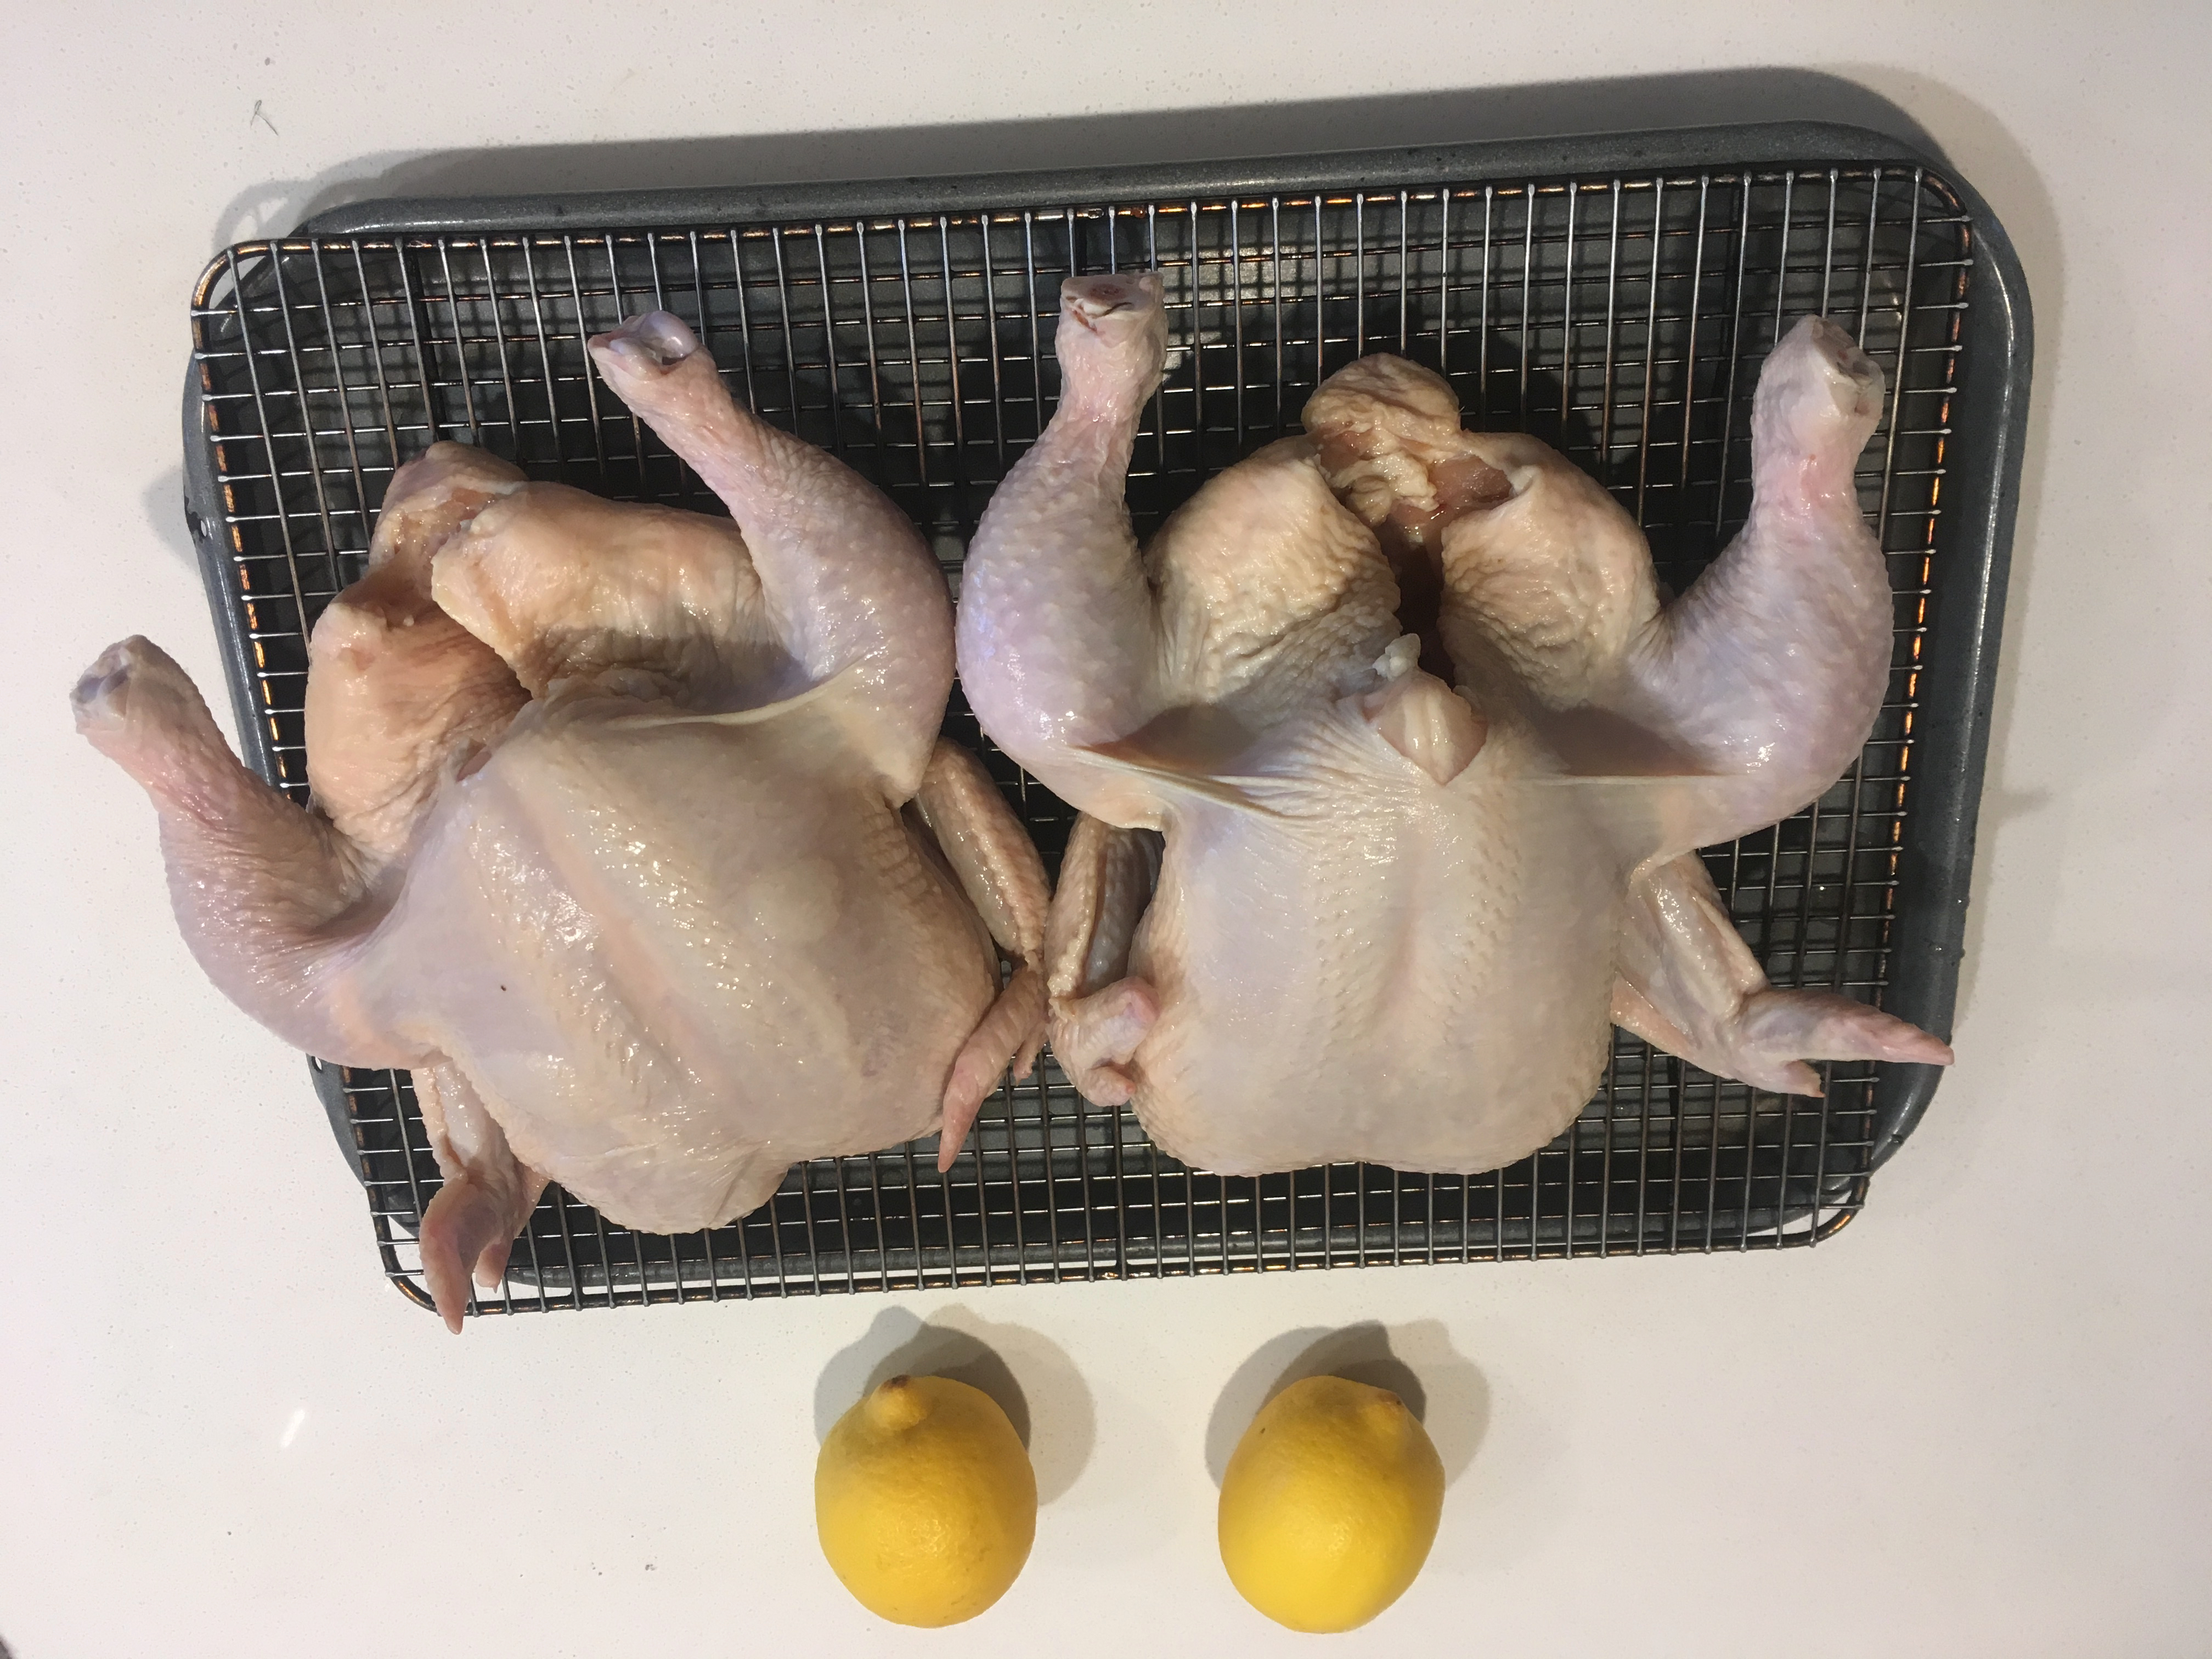
\includegraphics[width=0.25\textwidth]{\imageDir/\fileName/IMG_3197.jpg} &
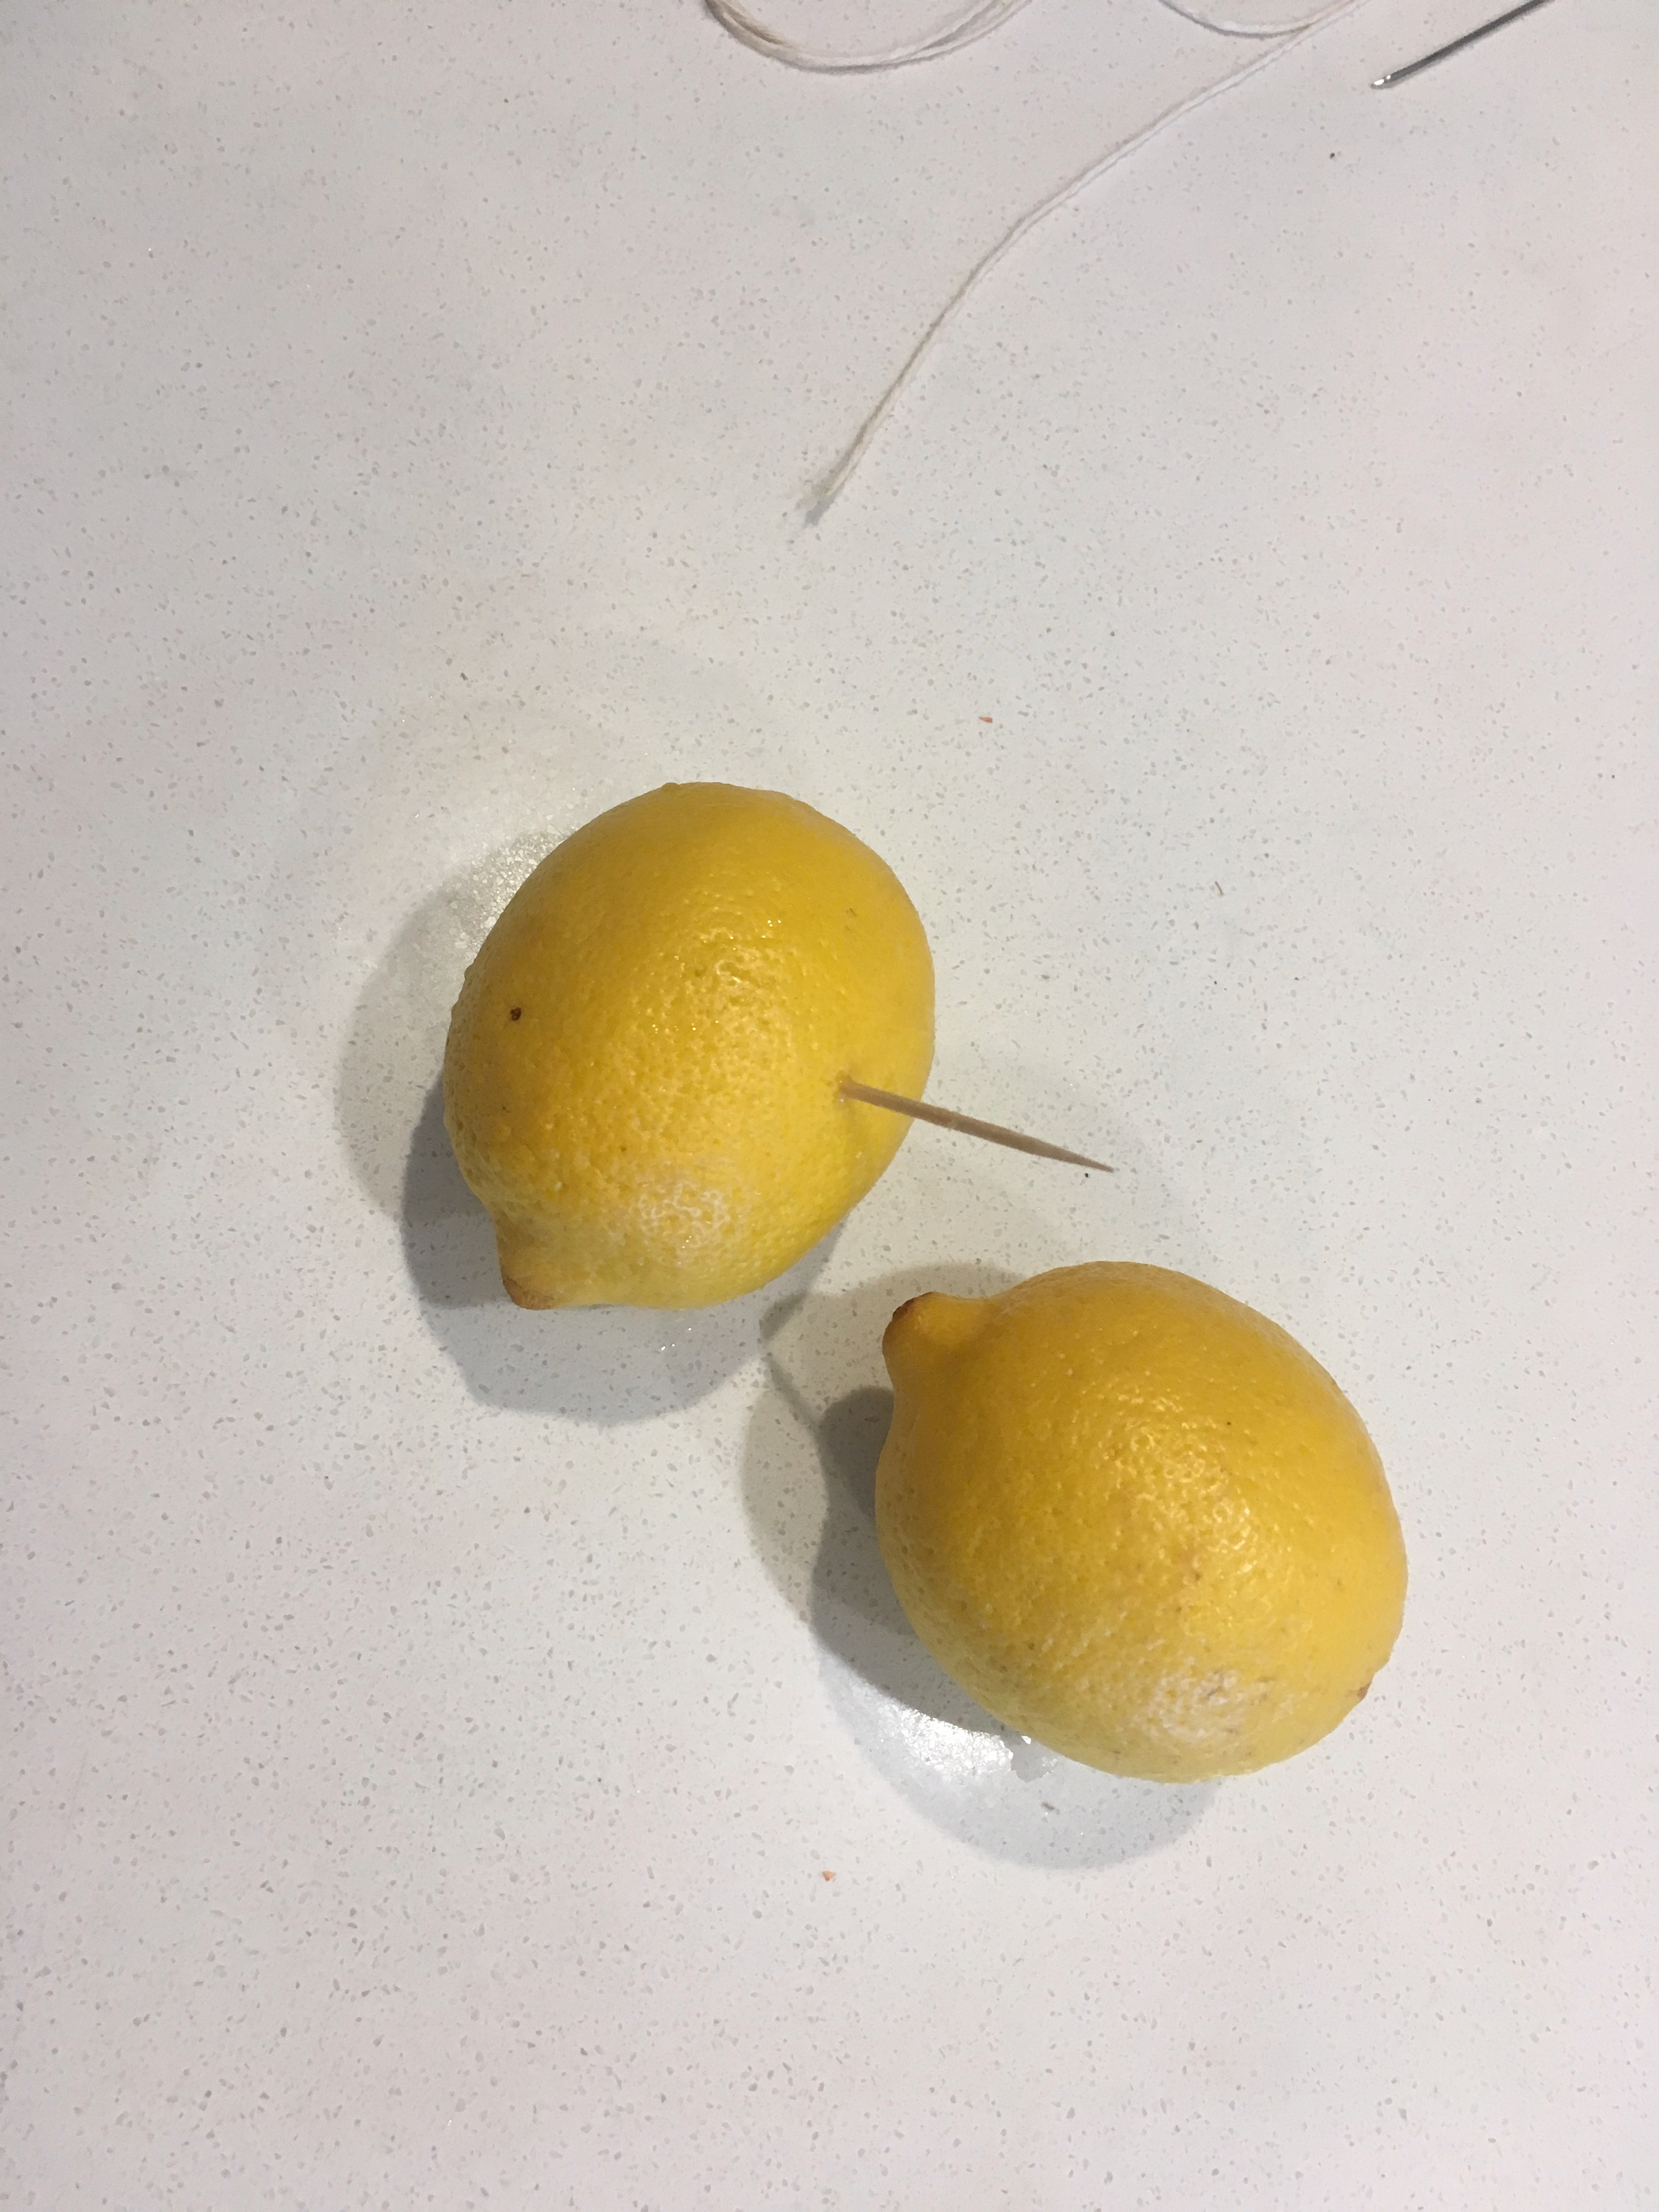
\includegraphics[width=0.25\textwidth]{\imageDir/\fileName/IMG_3212.jpg} &
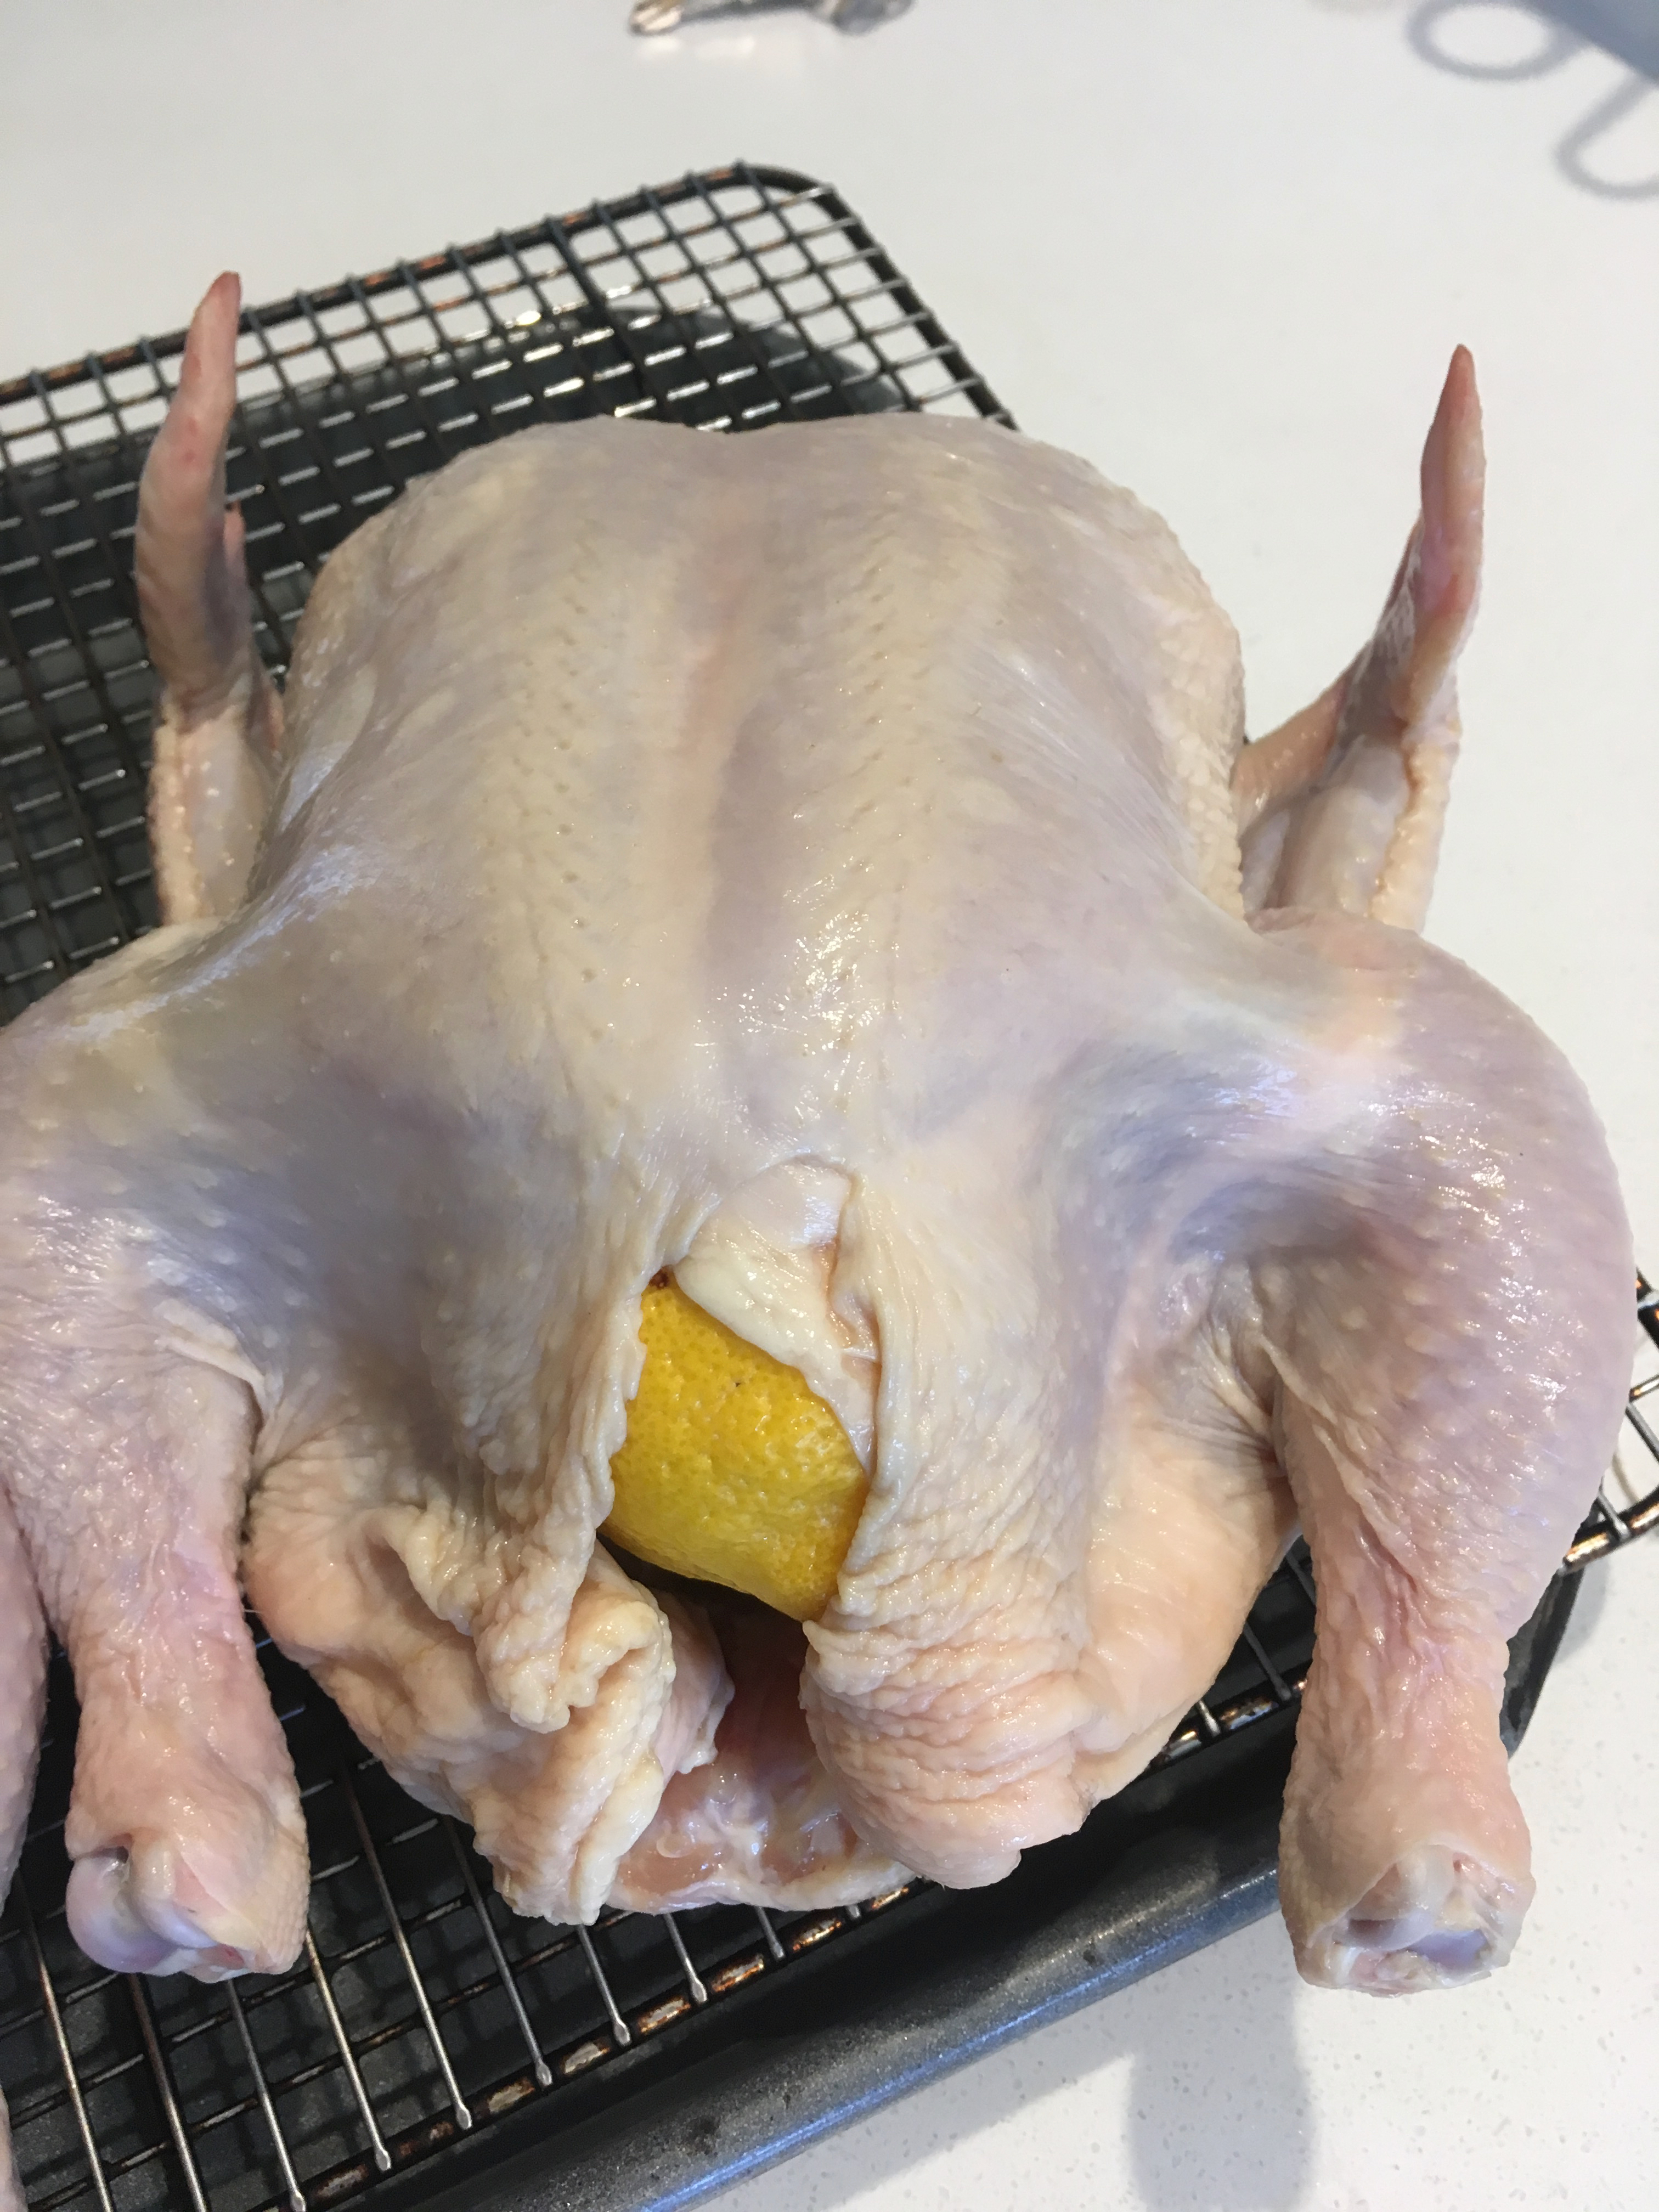
\includegraphics[width=0.25\textwidth]{\imageDir/\fileName/IMG_3213.jpg} \\
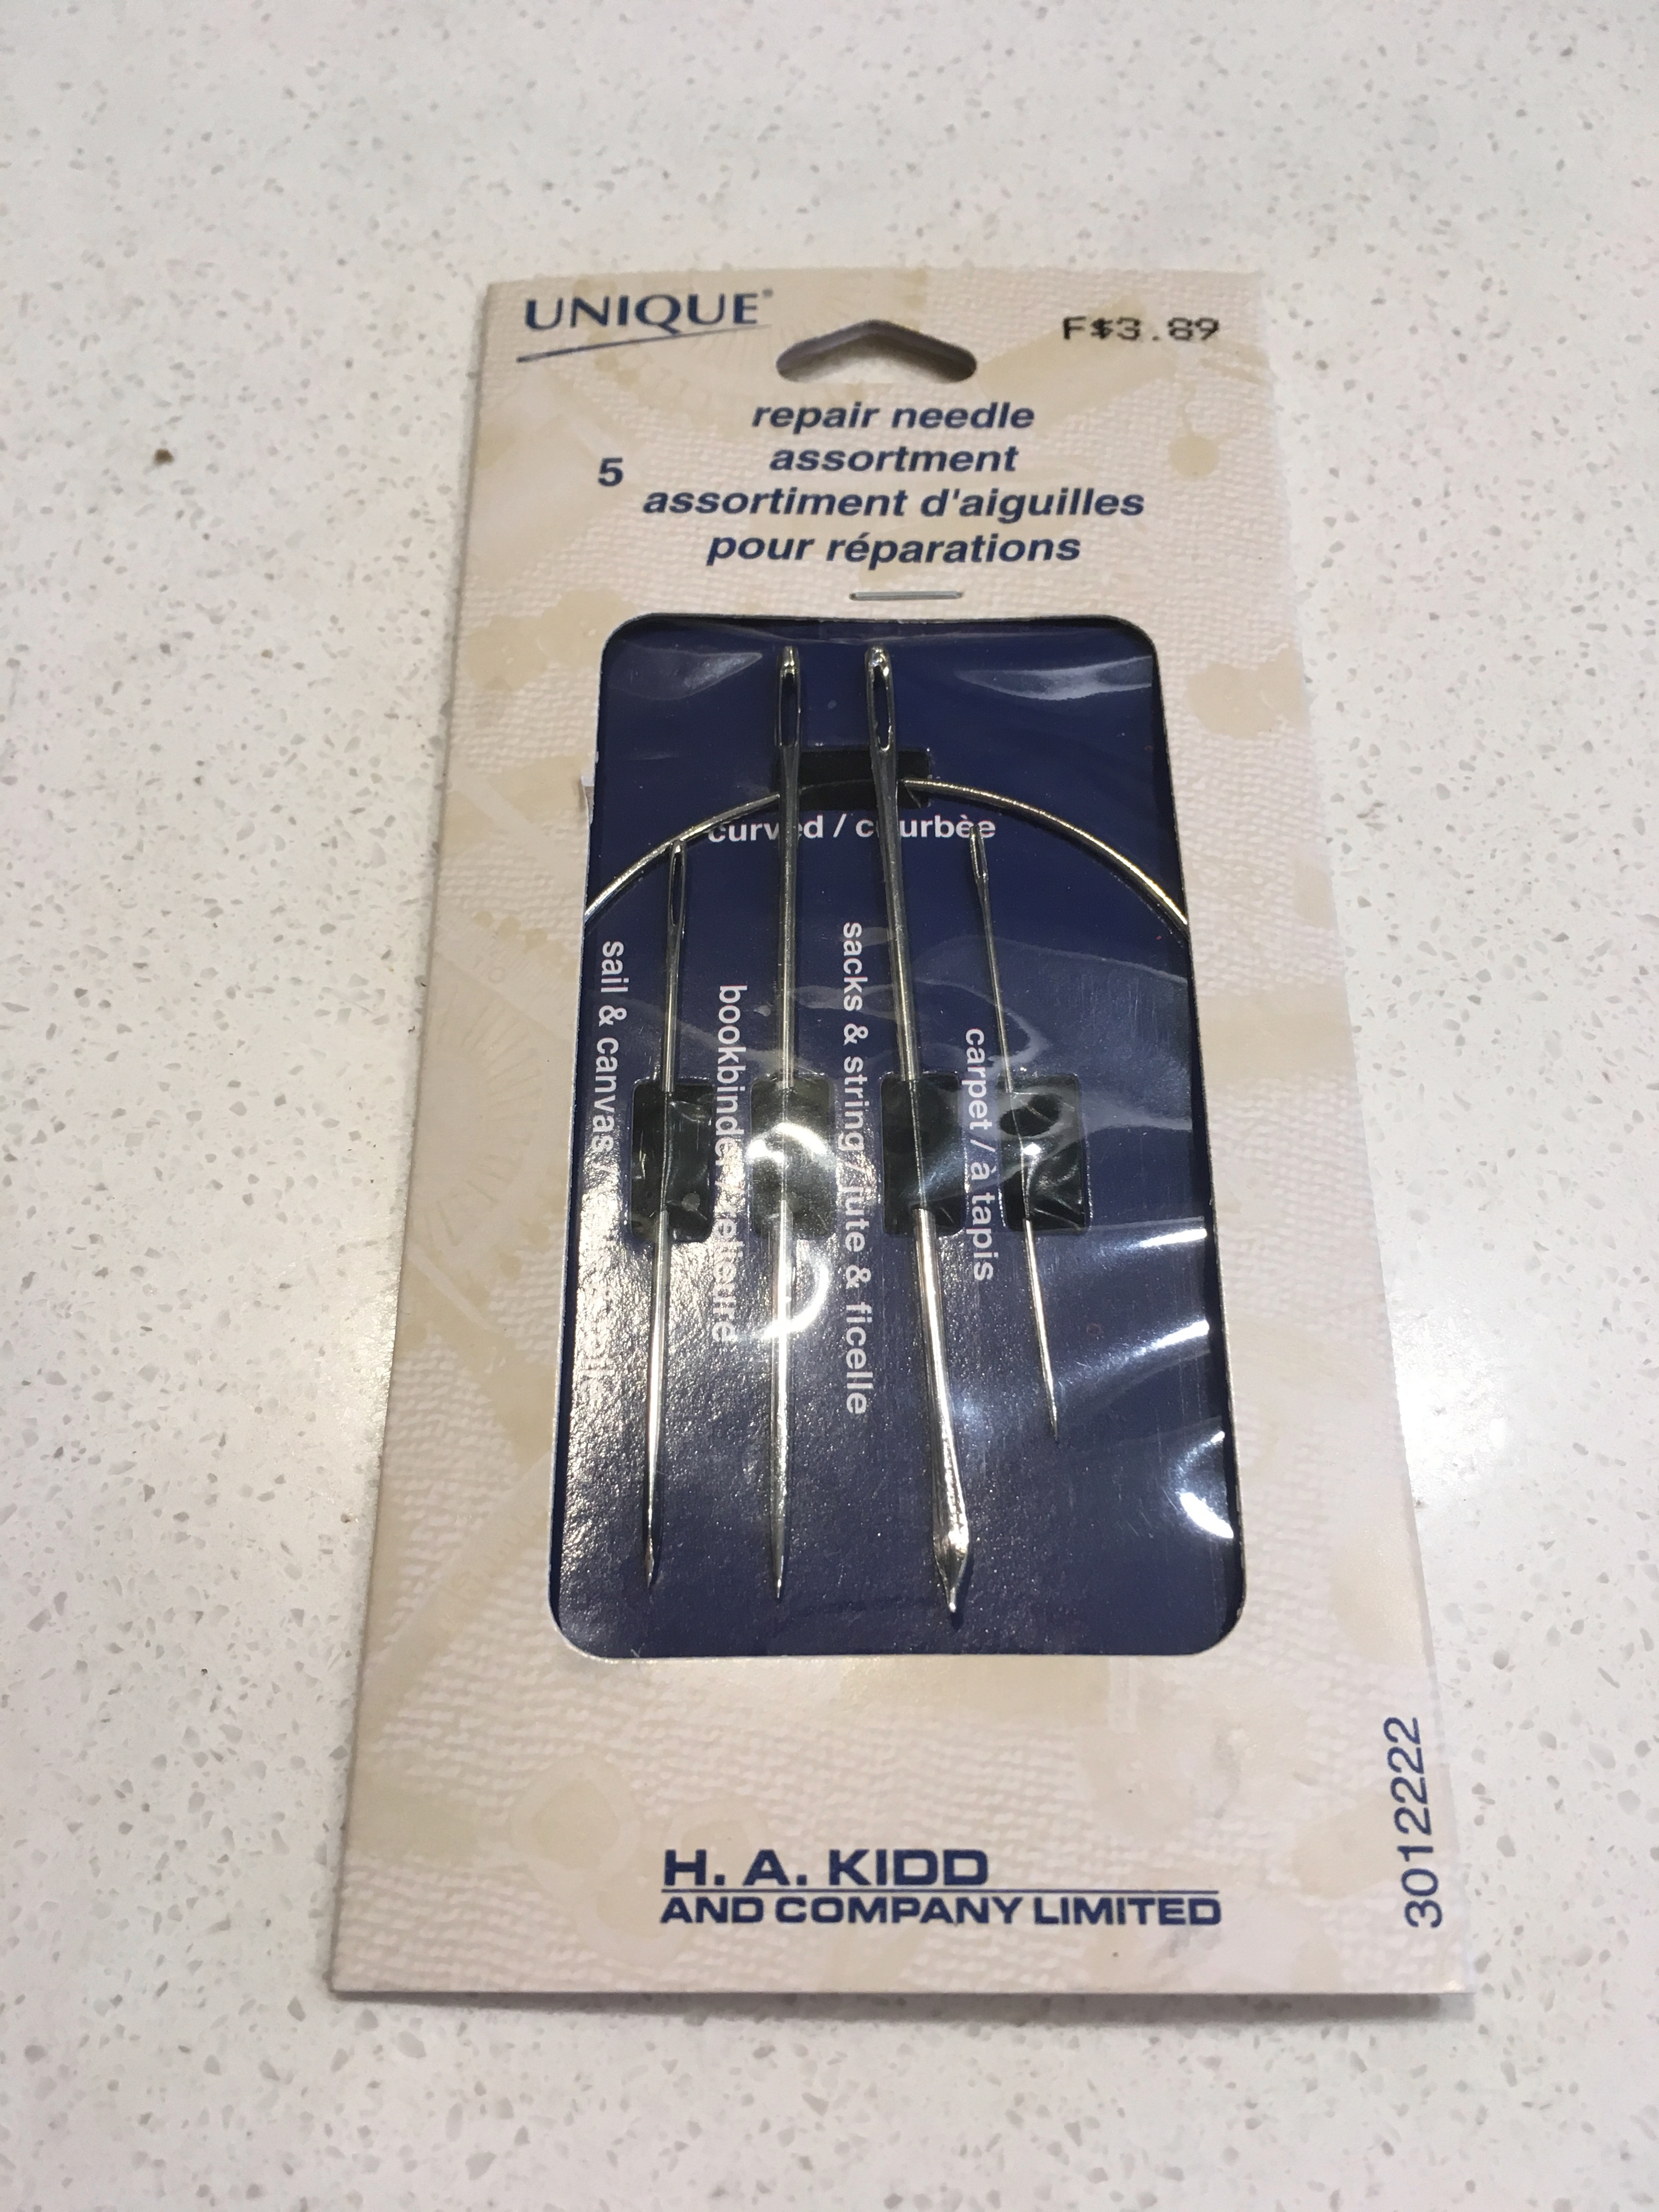
\includegraphics[width=0.25\textwidth]{\imageDir/\fileName/IMG_3206.jpg} &
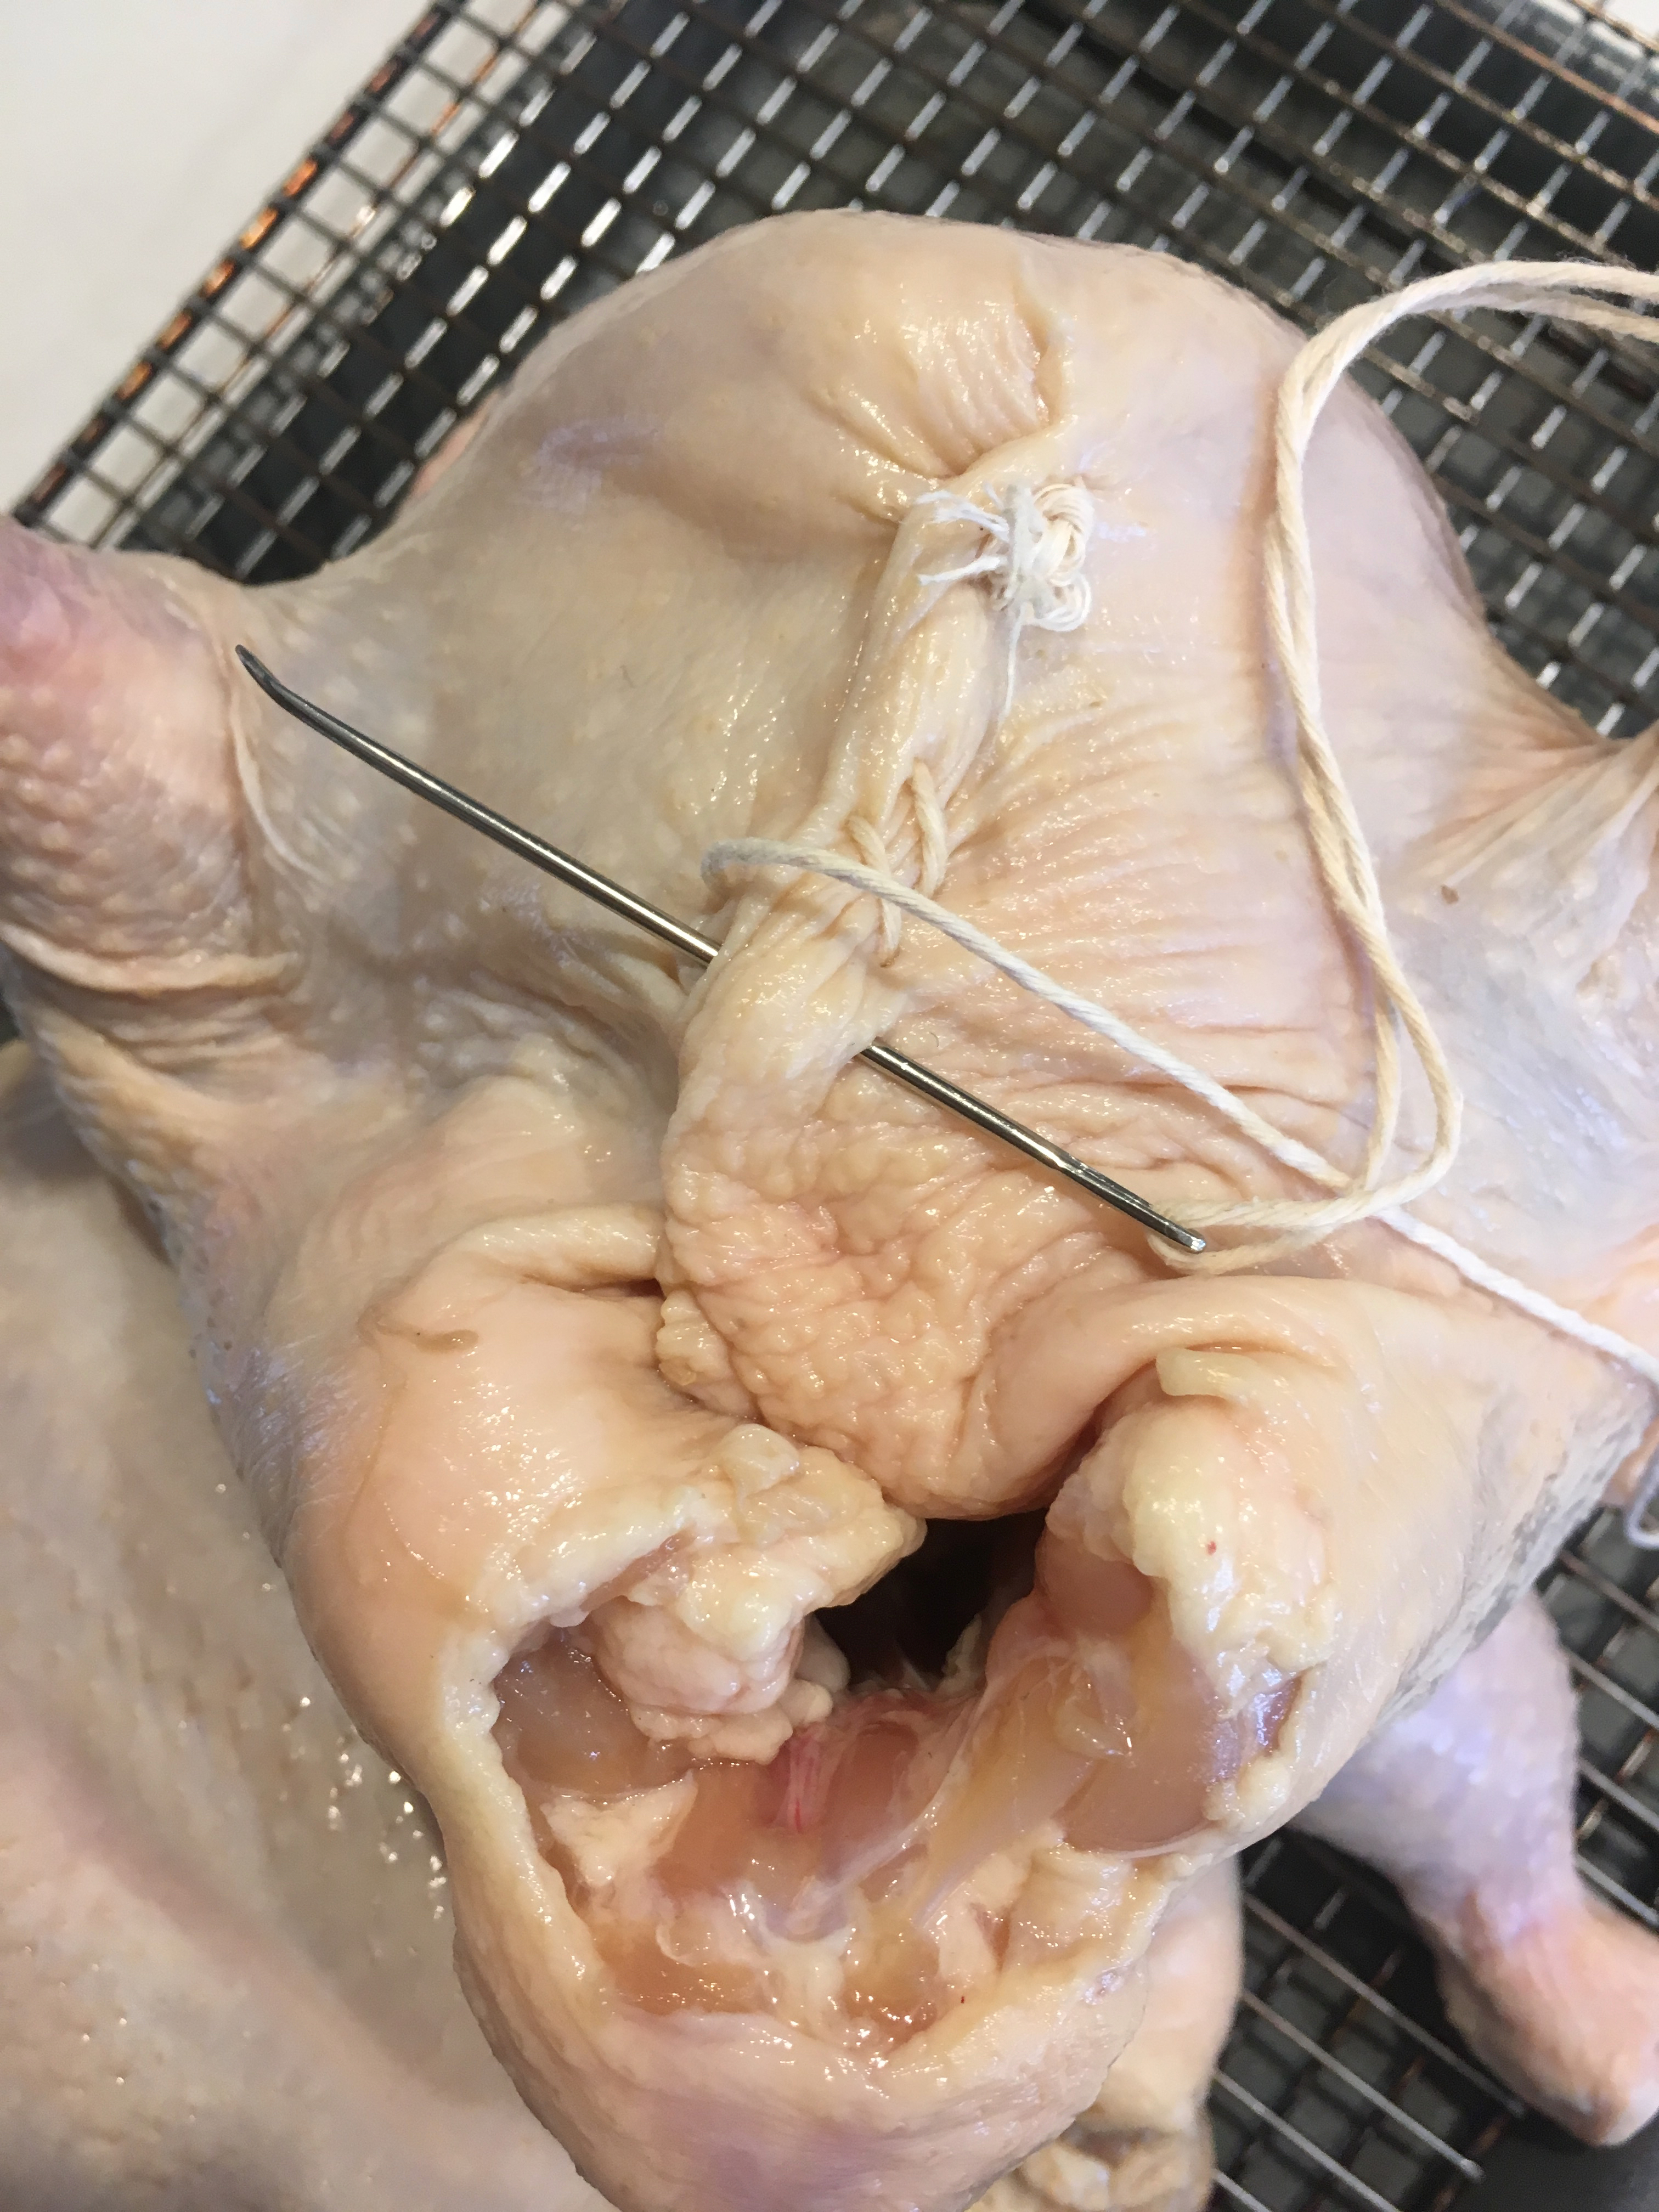
\includegraphics[width=0.25\textwidth]{\imageDir/\fileName/IMG_3214.jpg} &
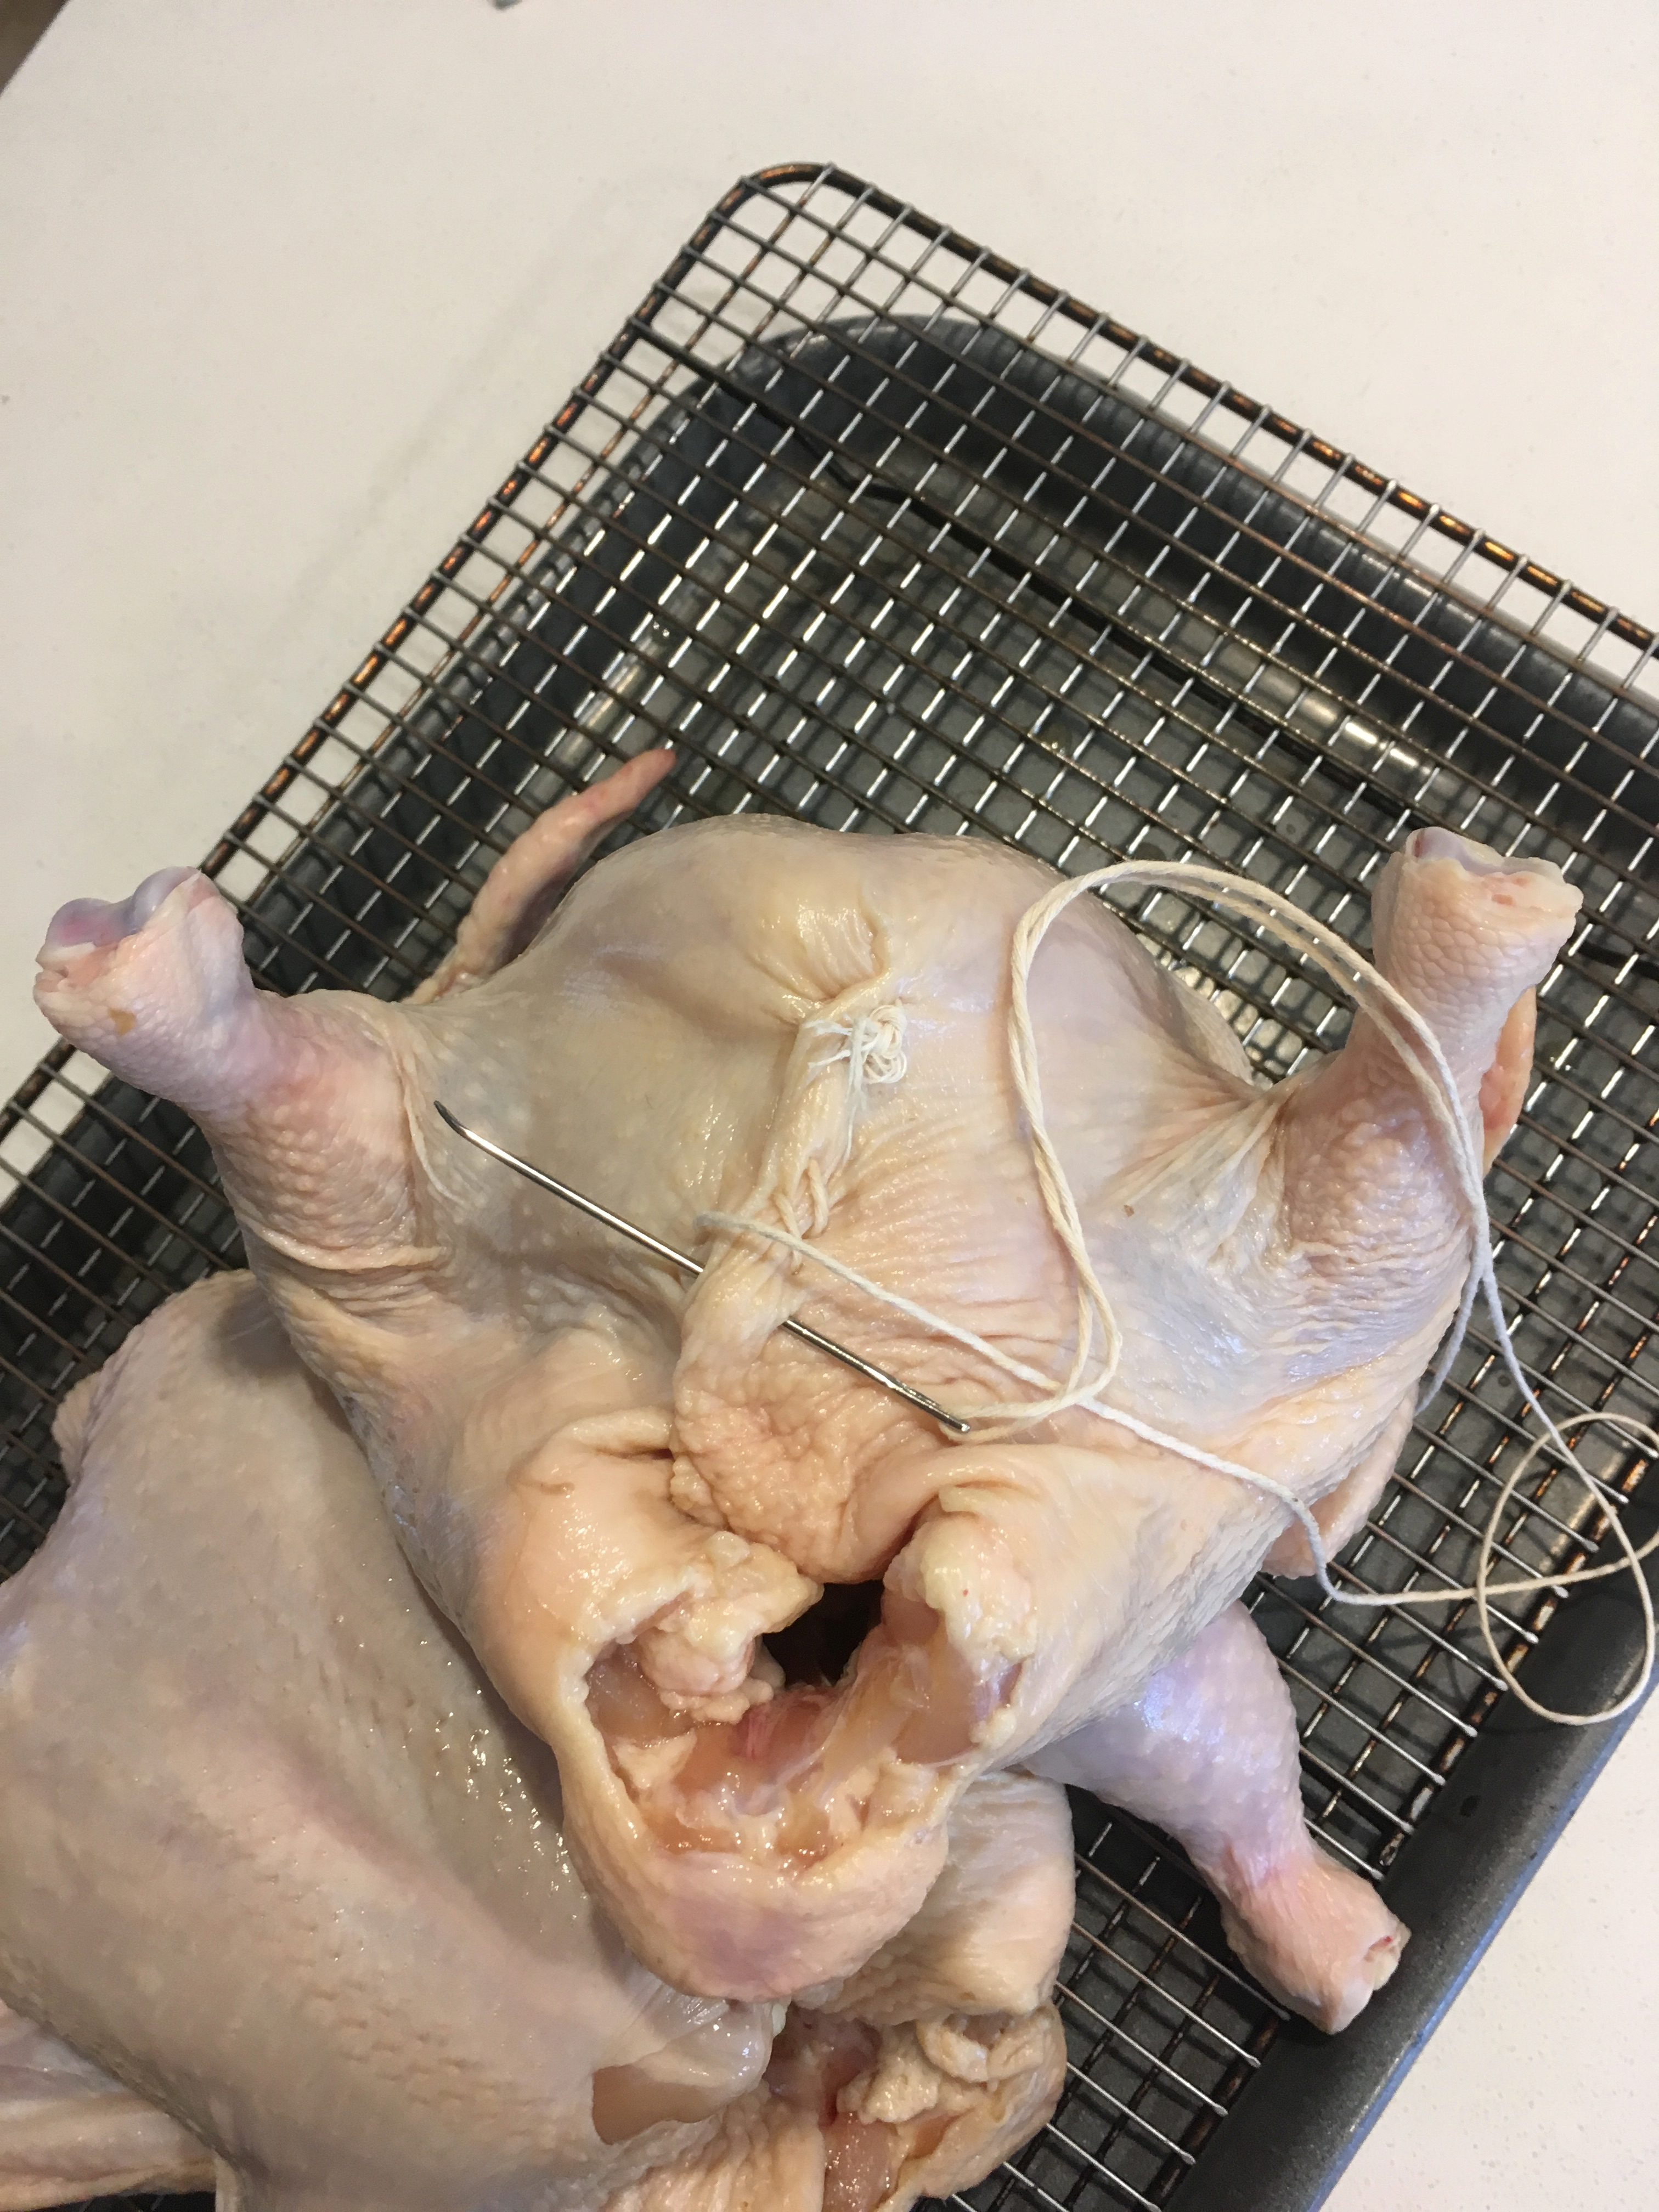
\includegraphics[width=0.25\textwidth]{\imageDir/\fileName/IMG_3216.jpg} \\
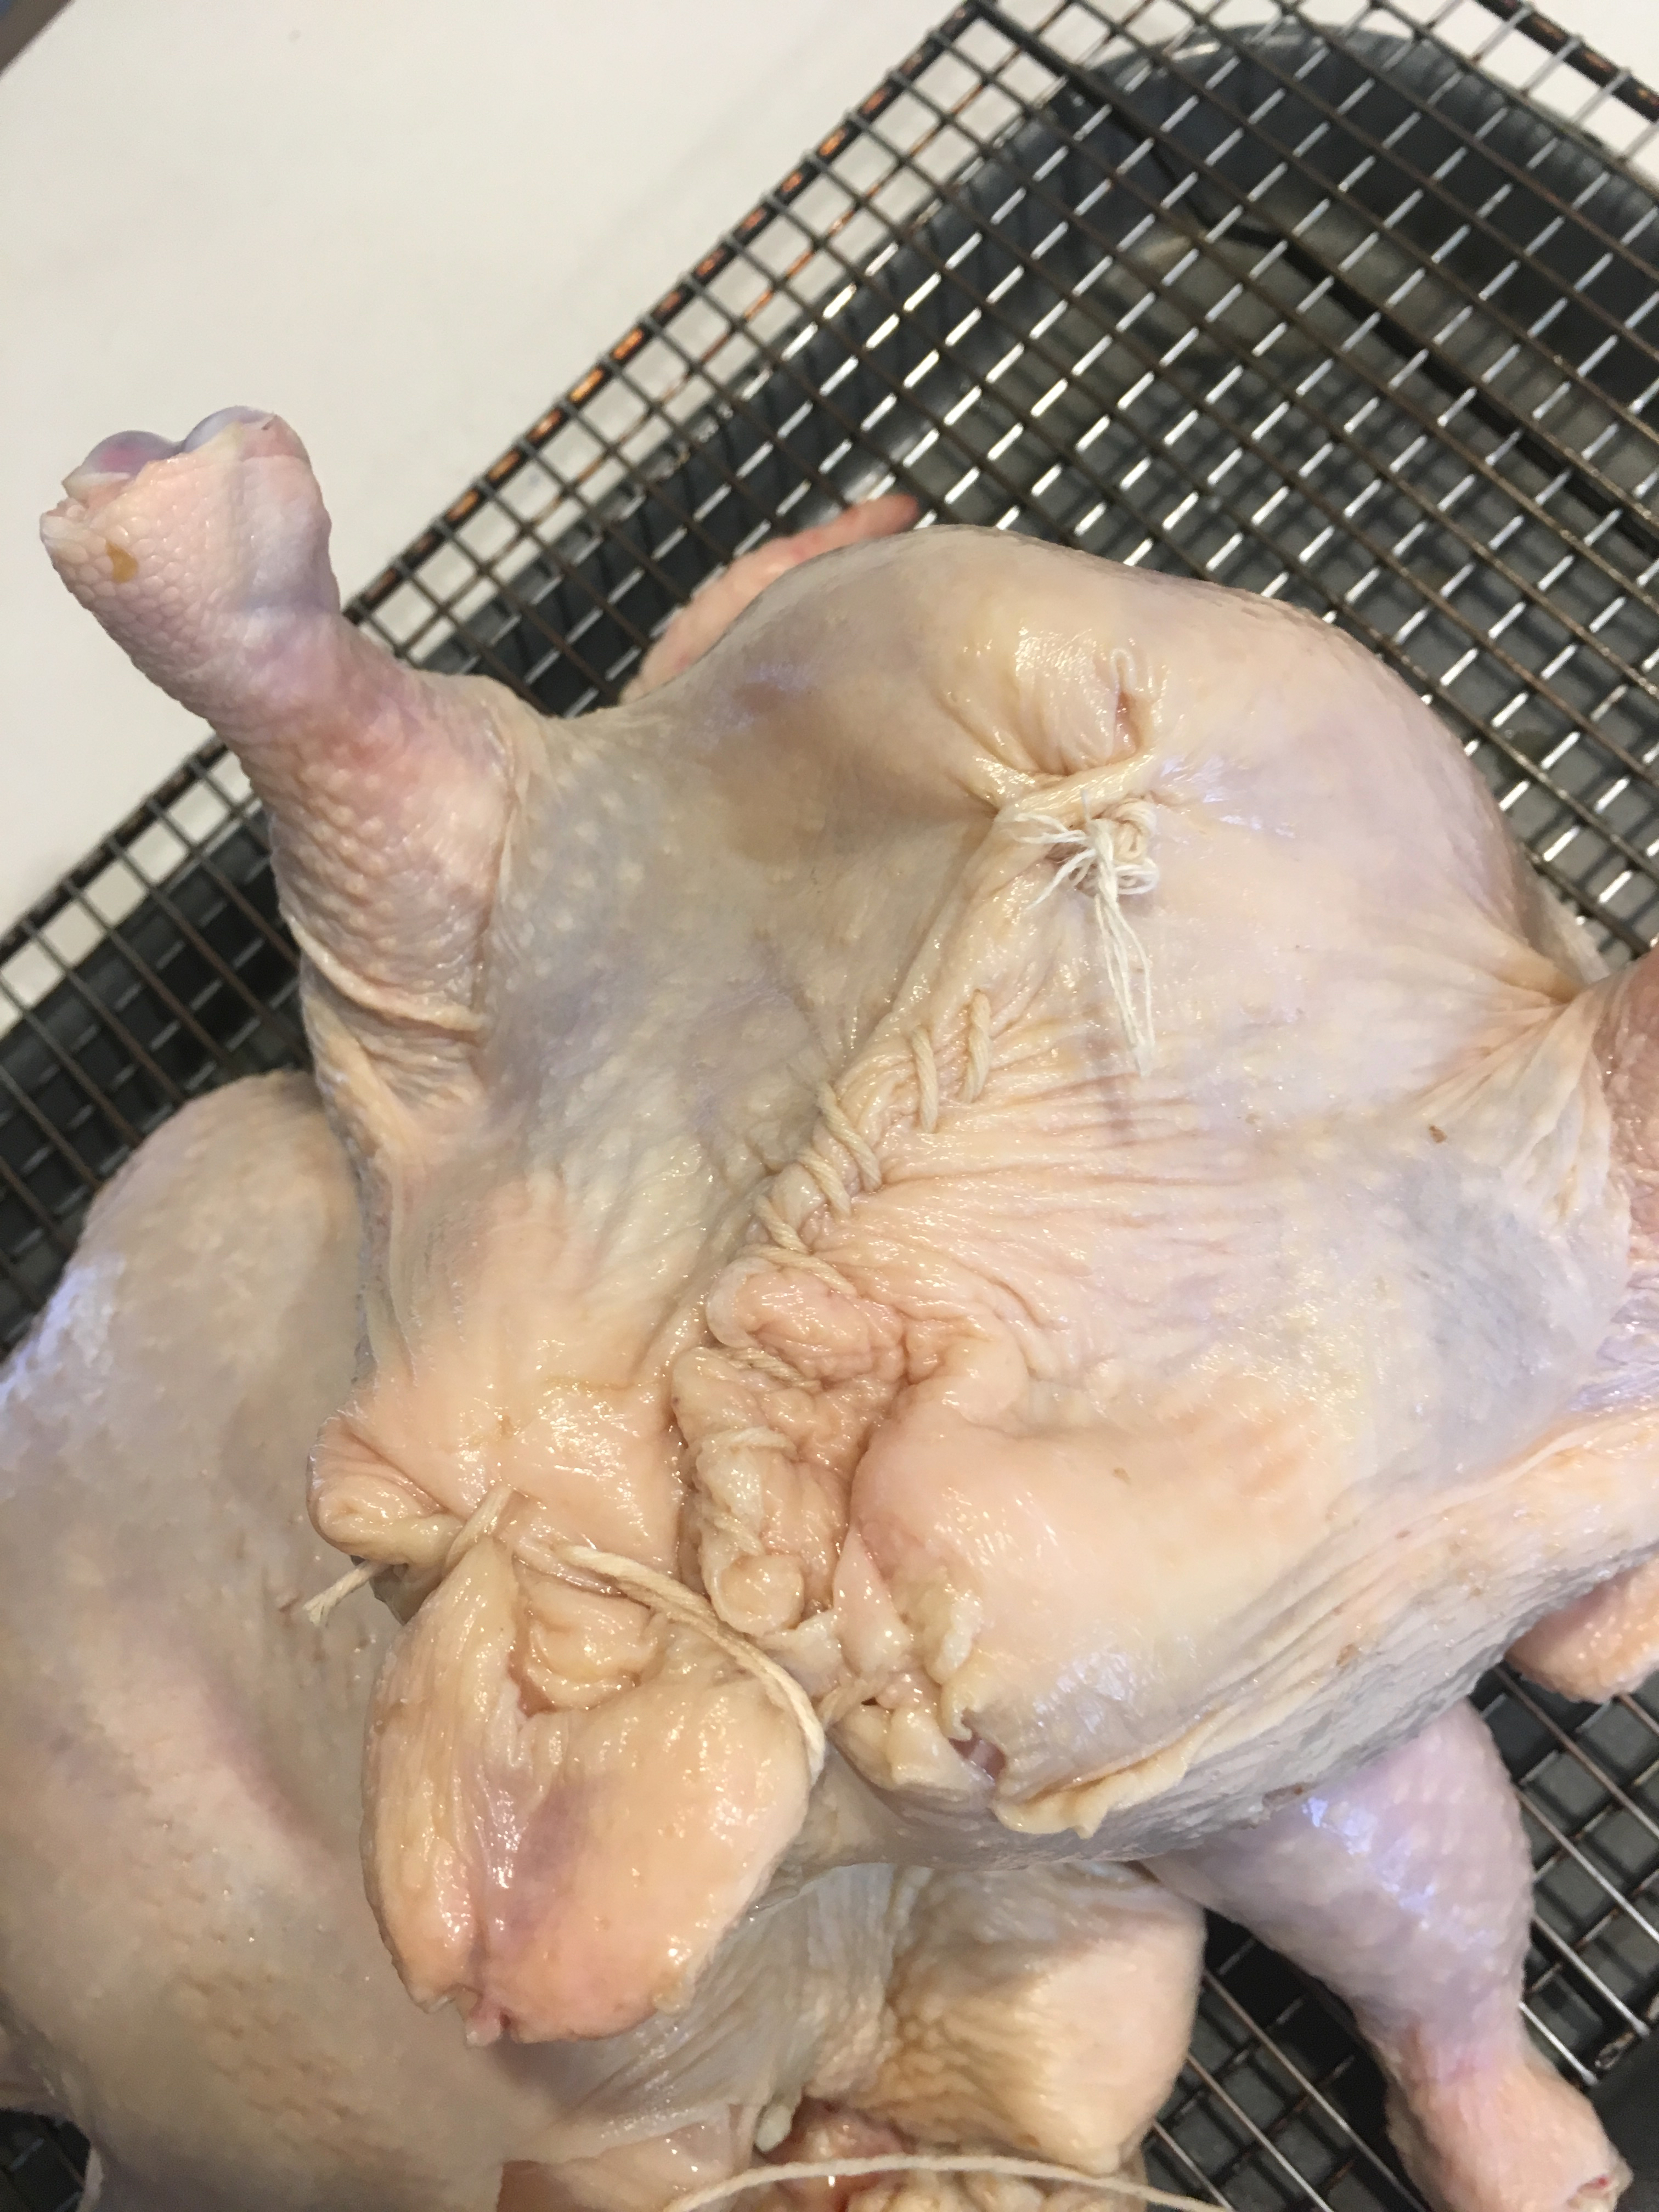
\includegraphics[width=0.25\textwidth]{\imageDir/\fileName/IMG_3217.jpg} &
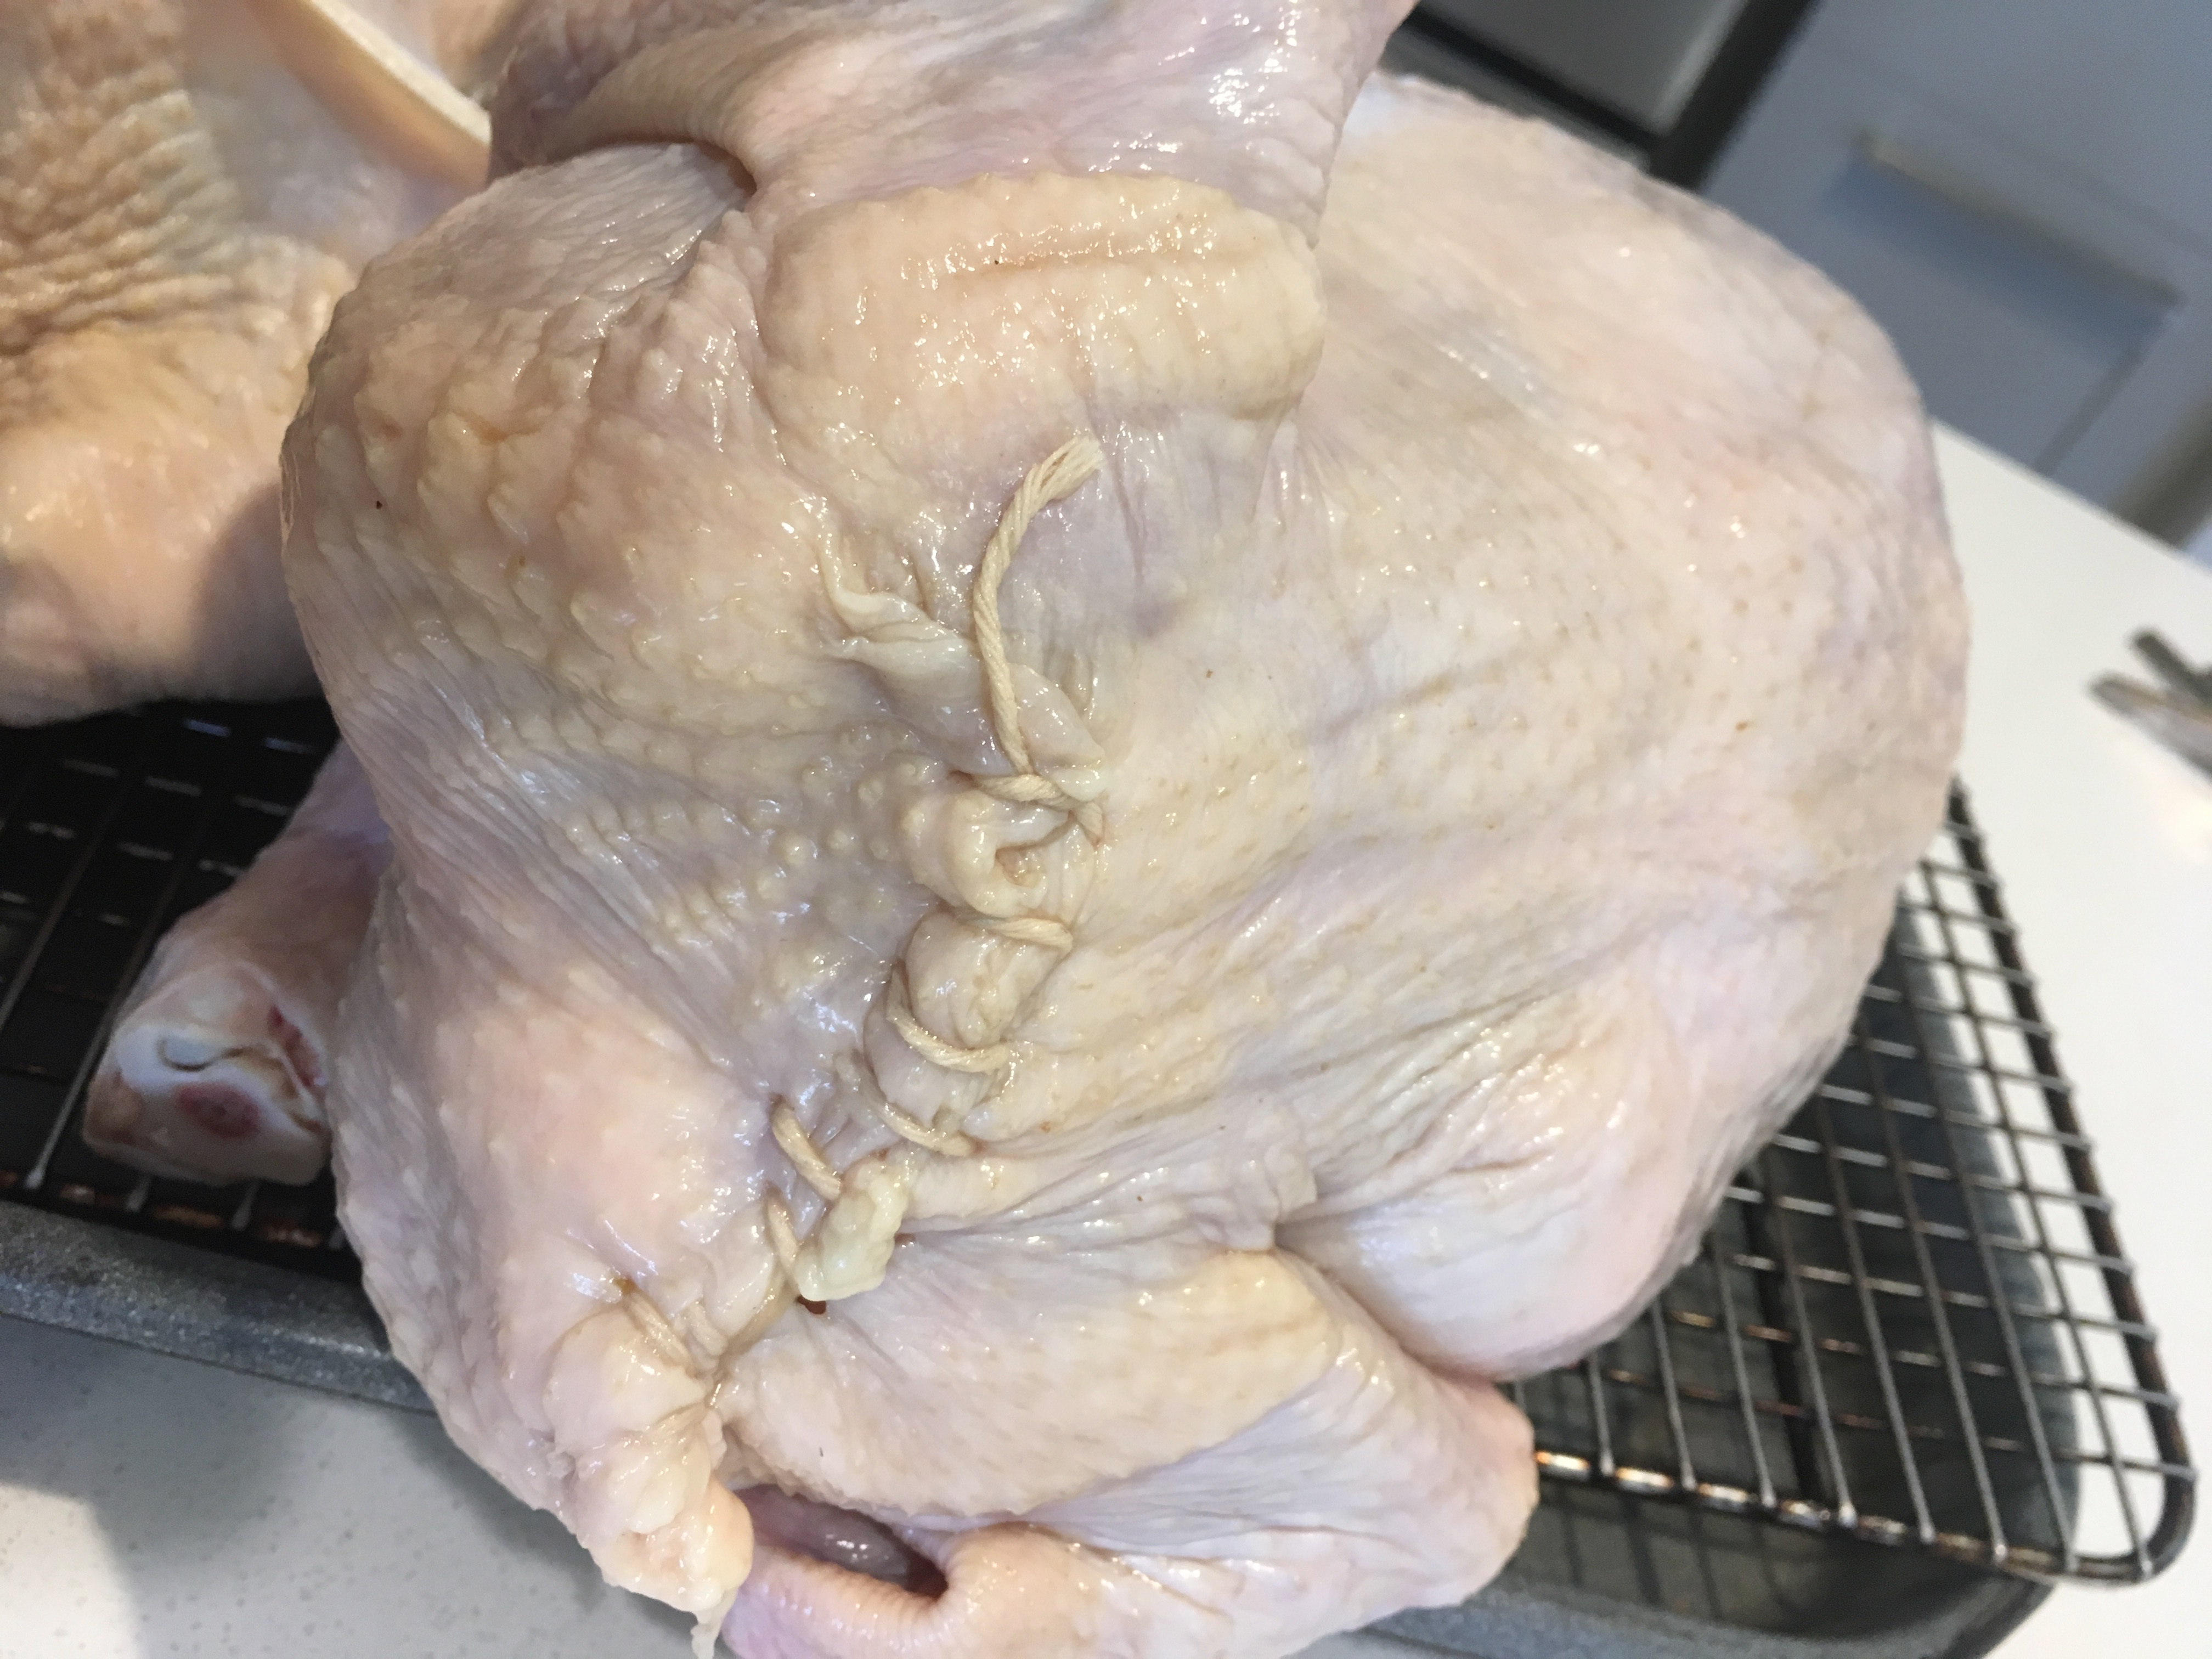
\includegraphics[width=0.25\textwidth]{\imageDir/\fileName/IMG_3218.jpg} &
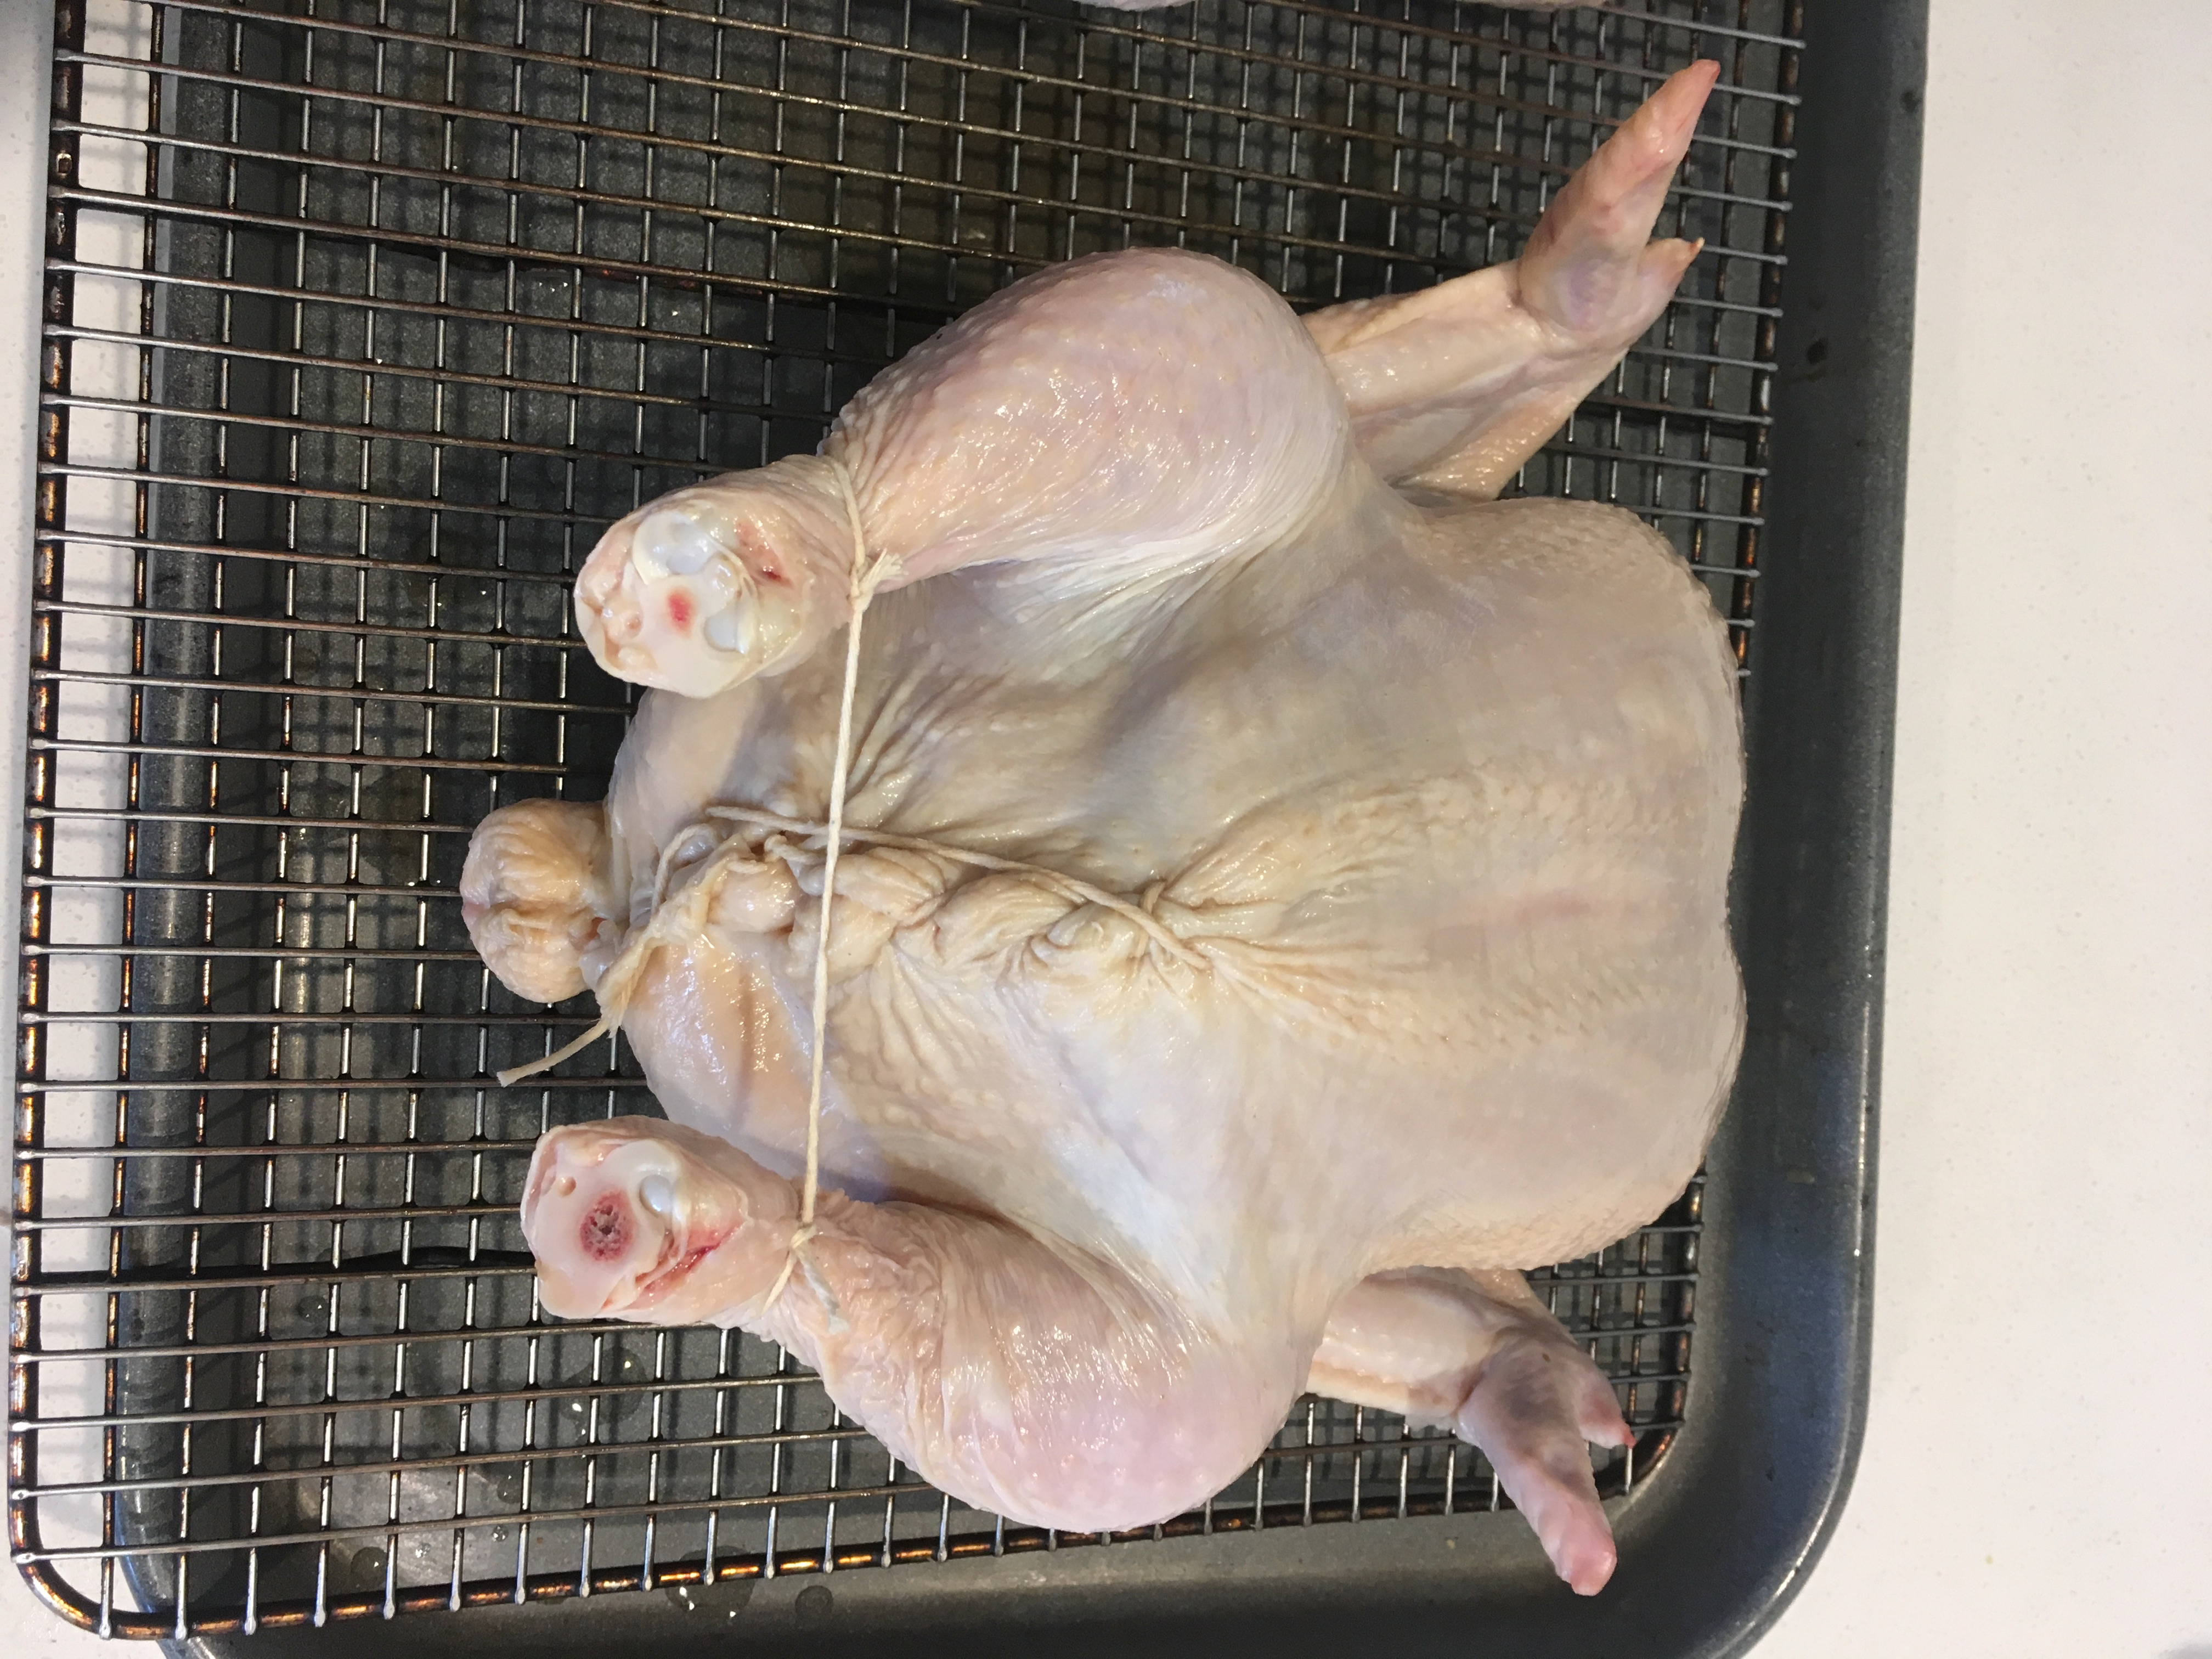
\includegraphics[width=0.25\textwidth]{\imageDir/\fileName/IMG_3219.jpg} \\
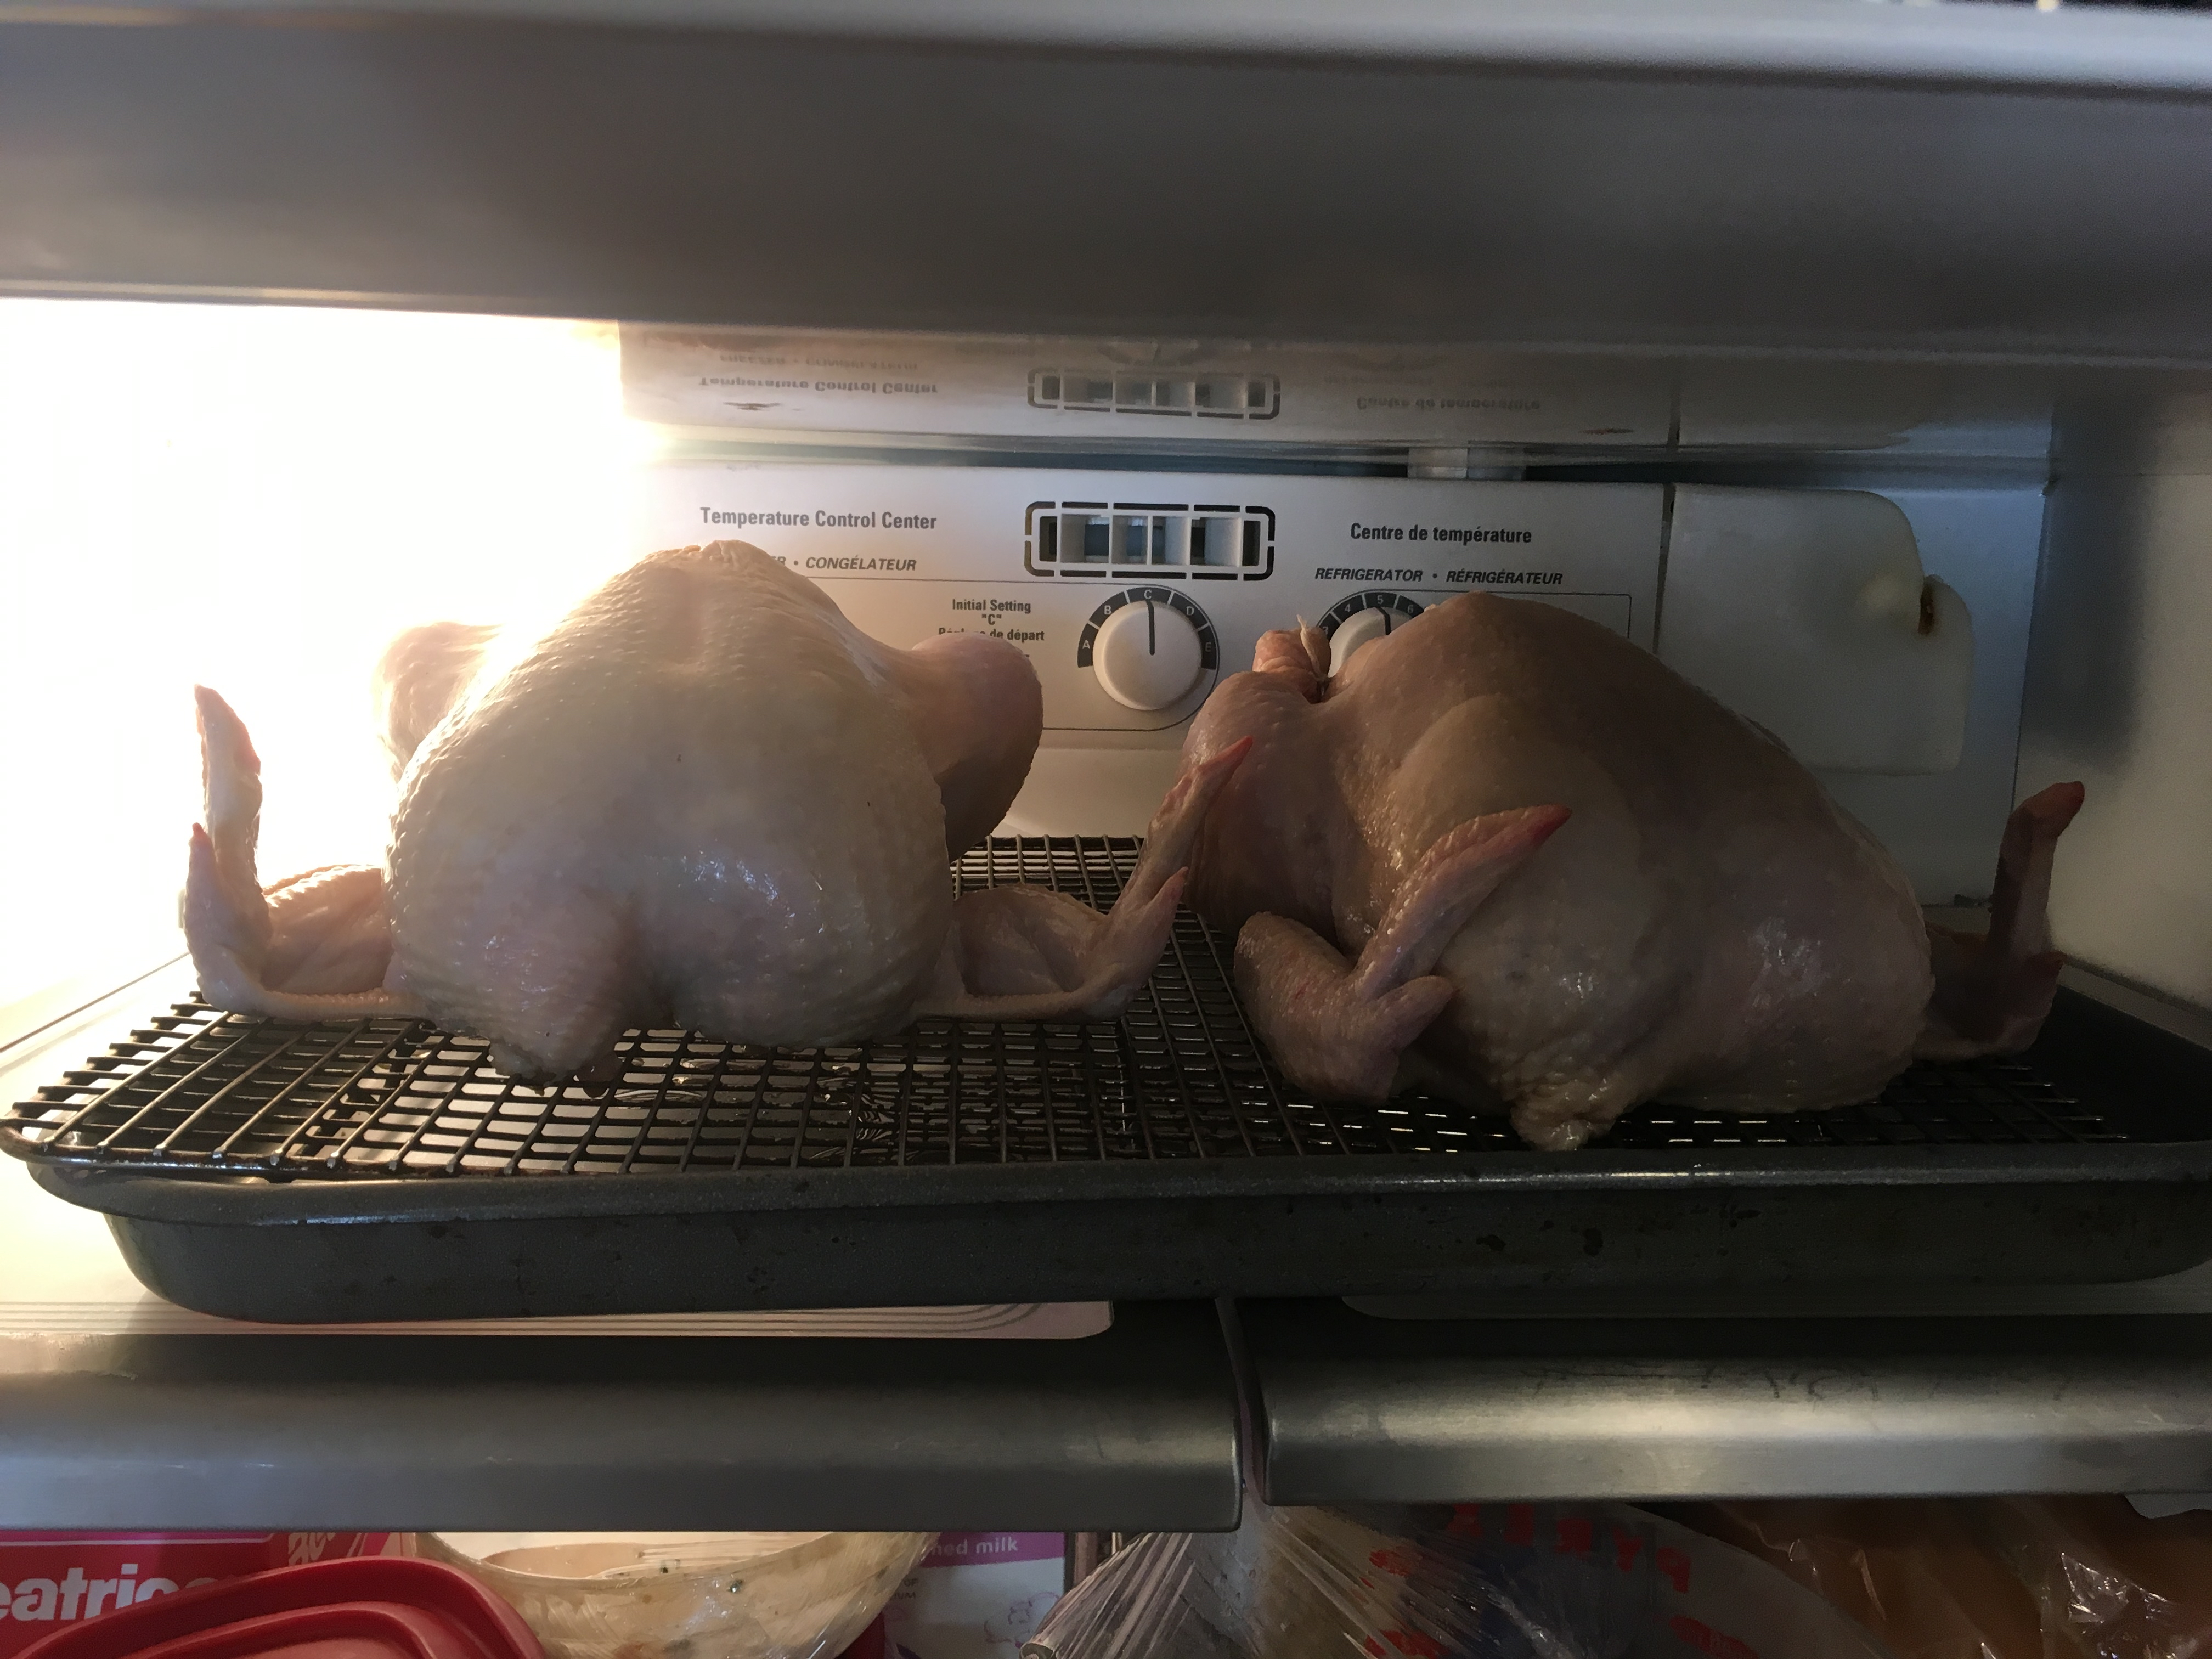
\includegraphics[width=0.25\textwidth]{\imageDir/\fileName/IMG_3220.jpg} &
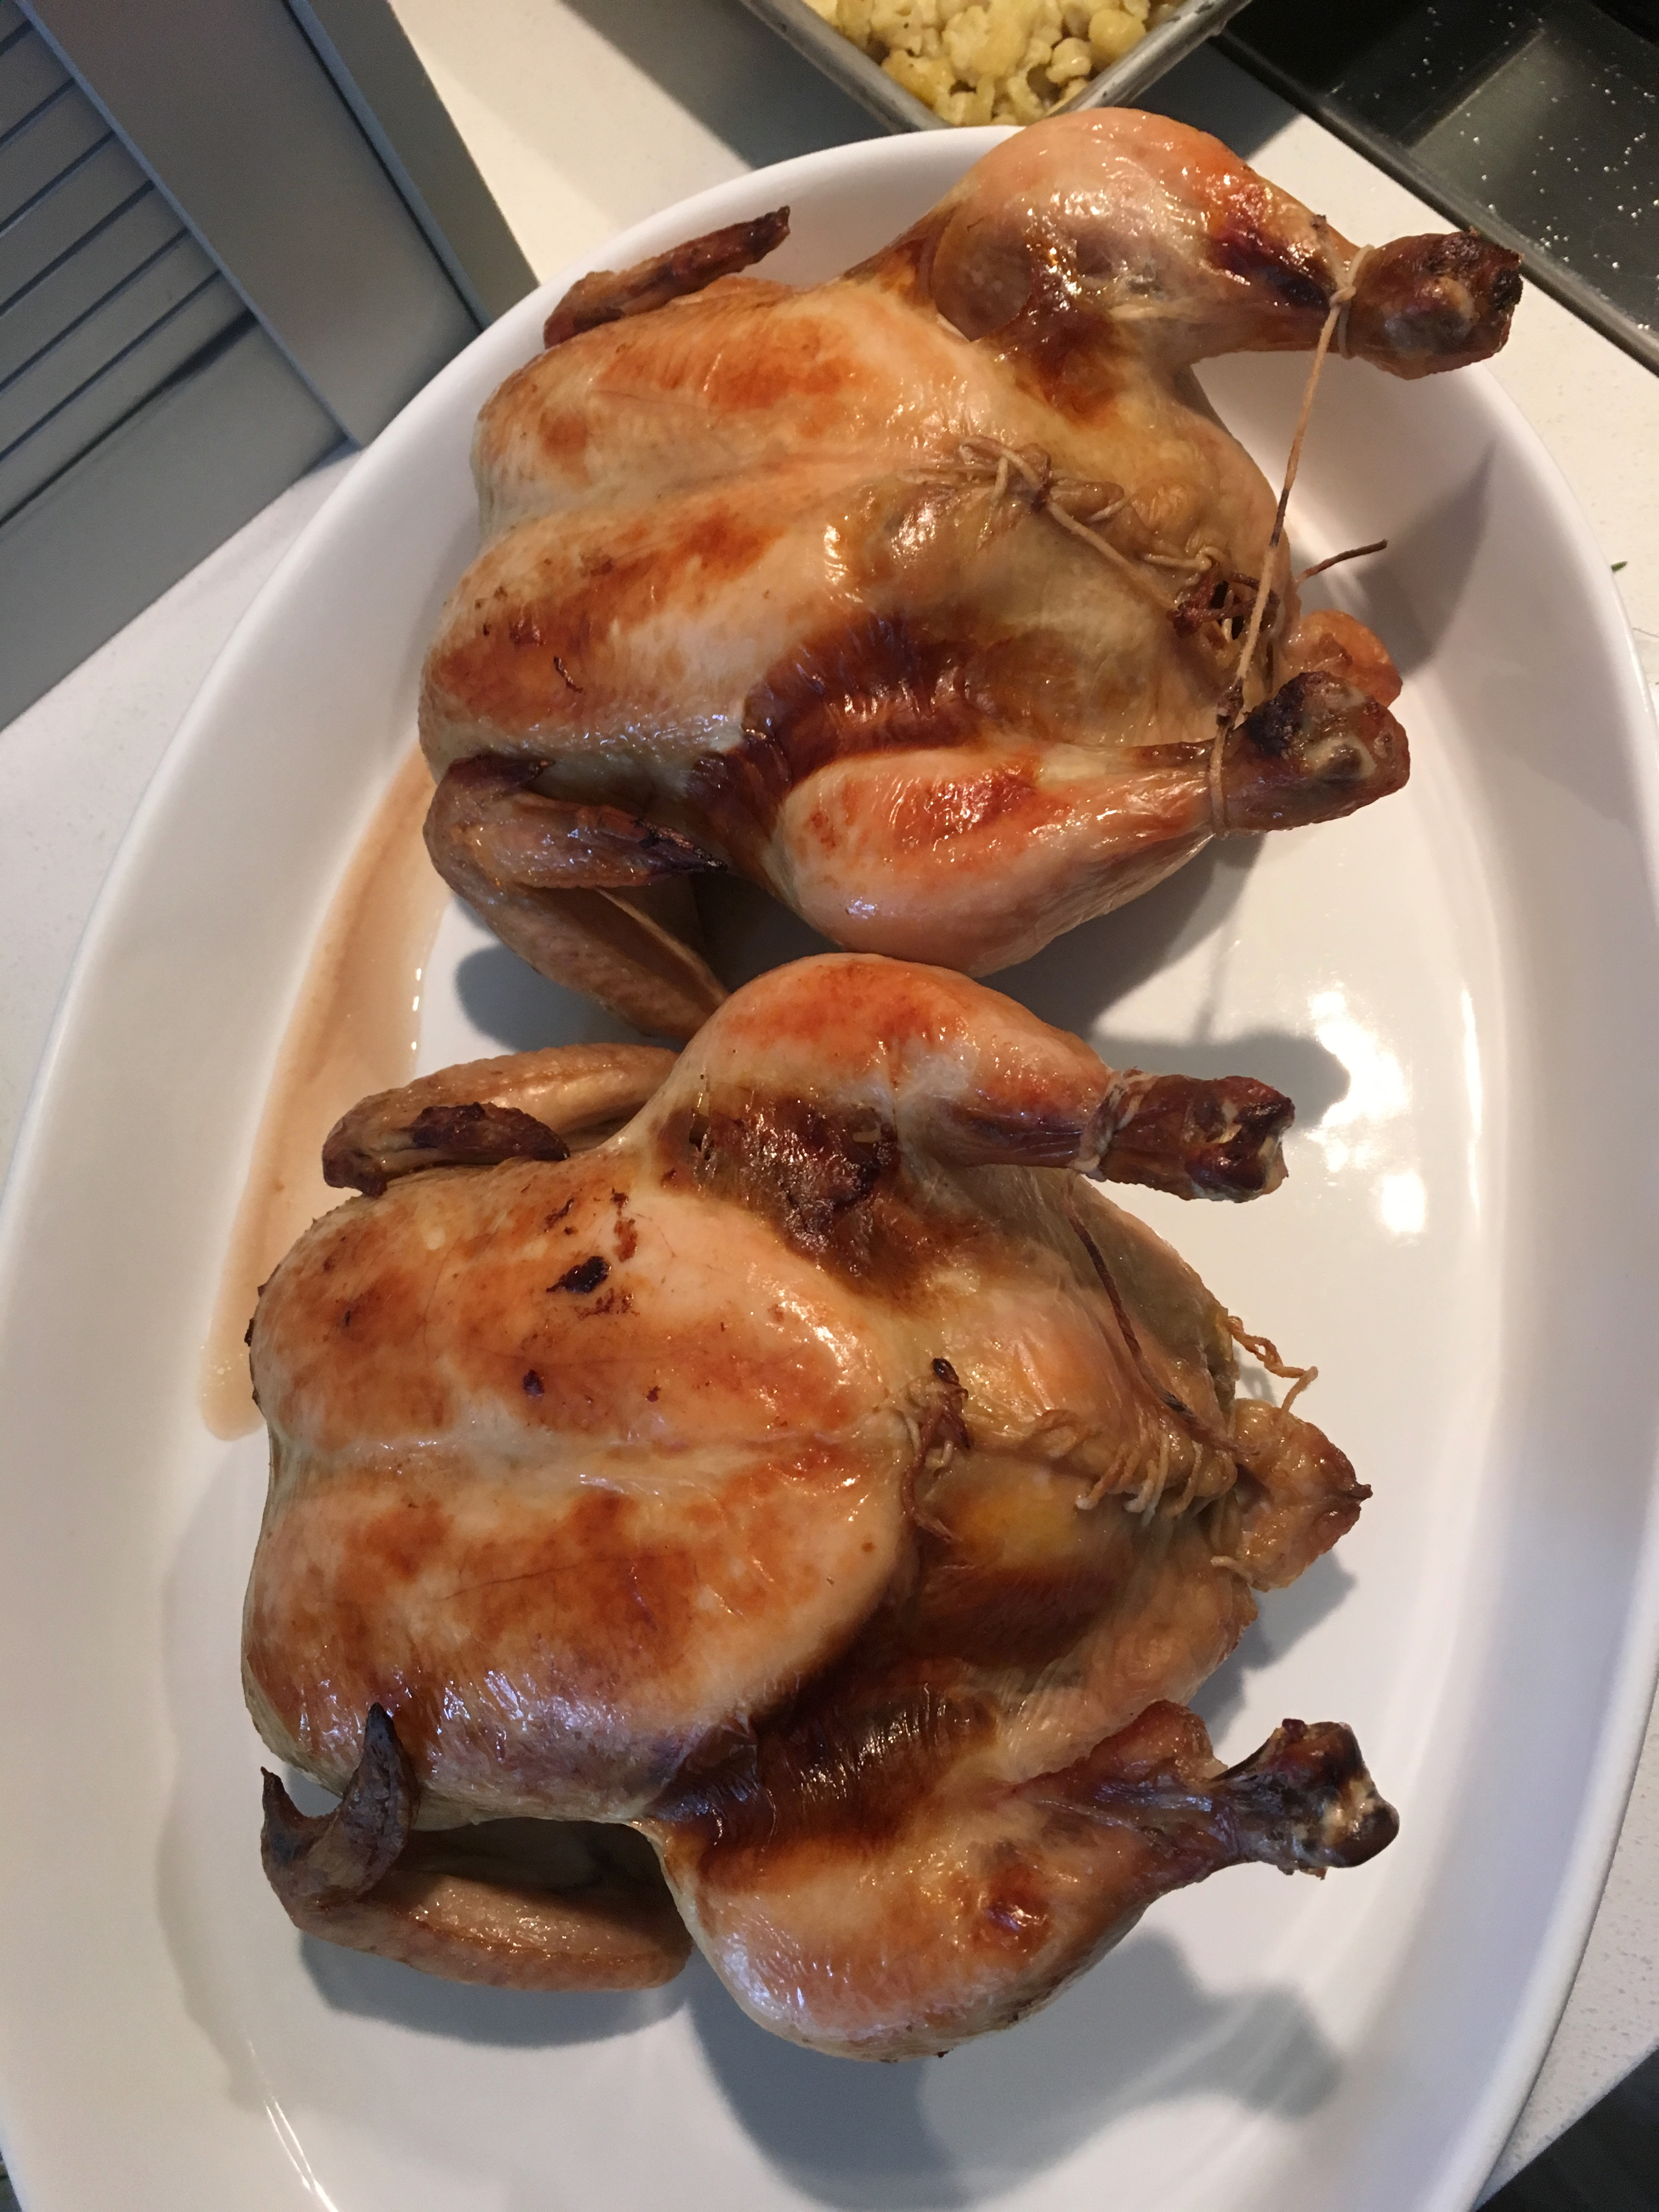
\includegraphics[width=0.25\textwidth]{\imageDir/\fileName/IMG_3228.jpg} \\
\end{tabular}
\end{table}


\end{document}
